\documentclass[newfonts=false, timestamp, format=sigplan, authordraft, 10pt,
letterpaper]{acmart}

%% \documentclass[sigplan, anonymous, screen, 10pt]{acmart}

\setcopyright{rightsretained}
\acmDOI{10.475/123_4}
\acmISBN{123-4567-24-567/08/06}
\acmConference[SIGCOMM'18]{ACM Special Interest Group on Data
  Communication}{August 2018}{Budapest, Hungary}
\acmYear{2018}
\copyrightyear{2018}
\acmPrice{15.00}

% \settopmatter{printacmref=false, printfolios=false}
% \renewcommand\footnotetextcopyrightpermission[1]{}
% \newcommand\eat[1]{}
% \pagestyle{plain}

\usepackage{times}

\usepackage[T1]{fontenc}
\usepackage[explicit]{titlesec}
\usepackage[font=small,labelfont=bf]{caption}
\usepackage[toc,page]{appendix}
\usepackage{algpseudocode}
\usepackage{amsmath}
\usepackage{amssymb}
\usepackage{balance}
\usepackage{booktabs} % For formal tables
\usepackage{enumitem}
\usepackage{hyperref}
\usepackage{listings}
\usepackage{microtype}
\usepackage{multirow}
\usepackage{siunitx}
\usepackage{subcaption}
\usepackage{tikz}
\usepackage{varwidth}
\usepackage{xcolor}

\hypersetup{
  colorlinks=true,
  linkcolor=ACMRed,
  urlcolor=ACMBlue,
  citecolor=ACMRed,
}

\lstset{
  captionpos=b,
  showspaces=false,
  showtabs=false,
  breaklines=true,
  showstringspaces=false,
  breakatwhitespace=true,
  escapeinside={(*@}{@*)},
  basicstyle=\footnotesize\ttfamily,
  columns=fullflexible,
  morekeywords={maybe_downsample, maybe_skip, maybe}
}

\captionsetup[lstlisting]{font={footnotesize}}
\renewcommand{\lstlistingname}{Example}

% \makeatletter
% \newcommand\appendix@section[1]{%
%   \refstepcounter{section}%
%   \orig@section*{Appendix \@Alph\c@section: #1}%
%   \addcontentsline{toc}{section}{Appendix \@Alph\c@section: #1}%
% }
% \let\orig@section\section
% \g@addto@macro\appendix{\let\section\appendix@section}
% \makeatother

% \newcommand*{\Appendixautorefname}{Appendix}

\frenchspacing

%%%%%%%%%%%%%%%%%%%%%%%%%%%%%%%%%%%%%%%%%%%%%%%%%%%%%%%%%%%%%%%
%% Paper setup
%%%%%%%%%%%%%%%%%%%%%%%%%%%%%%%%%%%%%%%%%%%%%%%%%%%%%%%%%%%%%%%

\newcommand{\sysname}{AWStream}
\newcommand{\para}[1]{\smallskip\noindent\textbf{#1}}
\newcommand{\paraf}[1]{\noindent\textbf{#1}}
\newcommand{\todo}[1]{{\color{ACMRed}\bf{TODO: #1}\normalfont}}
\newcommand{\fixme}[1]{{\color{ACMRed}\bf{FIXME: #1}\normalfont}}
\newcommand{\question}[1]{{\color{ACMRed}\footnotesize{Q: #1}\normalfont}}

\newcommand{\maybe}{\texttt{maybe}}

\def\Snospace~{\S{}}
\renewcommand*\sectionautorefname{\Snospace}
\renewcommand*\subsectionautorefname{\Snospace}
\renewcommand*\subsubsectionautorefname{\Snospace}
\renewcommand*{\equationautorefname}{Eq.}
\renewcommand*{\figureautorefname}{Fig.}

\newcommand{\specialcell}[2][c]{%
  \begin{tabular}[#1]{@{}c@{}}#2\end{tabular}}

\newcommand*\circled[1]{\tikz[baseline=(char.base)]{
    \node[shape=circle,draw,inner sep=0.5pt] (char) {#1};}}

\newcommand*\qe{$\text{Q}_\text{E}$}
\newcommand*\qc{$\text{Q}_\text{C}$}
\newcommand*\rc{$\text{R}_\text{C}$}
\newcommand*\spd{$\text{S}_\text{ProbeDone}$}

%%% Local Variables:
%%% mode: latex
%%% TeX-master: "awstream"
%%% End:


\title{\sysname{}: Adaptive Wide-Area Streaming Analytics}
%% \gdef\addresses{Paper \textbf{\#104}, 12 pages}

\author{Ben Zhang}
\affiliation{UC Berkeley}
\email{benzh@cs.berkeley.edu}

\author{Xin Jin}
\affiliation{Johns Hopkins University}
\email{xinjin@cs.jhu.edu}

\author{Sylvia Ratnasamy}
\affiliation{UC Berkeley}
\email{sylvia@eecs.berkeley.edu}

\author{John Wawrzynek}
\affiliation{UC Berkeley}
\email{johnw@eecs.berkeley.edu}

\author{Edward A. Lee}
\affiliation{UC Berkeley}
\email{eal@eecs.berkeley.edu}

\renewcommand{\shortauthors}{B. Zhang et al.}

\begin{document}

\begin{abstract}

The emerging class of wide-area streaming analytics faces the challenge of
scarce and variable WAN bandwidth. Non-adaptive applications built with TCP or
UDP suffer from increased latency or degraded accuracy. State-of-the-art
approaches that adapt to network changes require developer writing sub-optimal
manual policies or are limited to application-specific optimizations.

We present \sysname{}, a stream processing system that simultaneously achieves
low latency and high accuracy in the wide area, requiring minimal developer
efforts. To realize this, \sysname{} uses three ideas: $(i)$ it integrates
application adaptation as a first-class programming abstraction in the stream
processing model; $(ii)$ with a combination of offline and online profiling, it
automatically learns an accurate profile that models accuracy and bandwidth
trade-off; and $(iii)$ at runtime, it carefully adjusts the application data
rate to match the available bandwidth while maximizing the achievable
accuracy. We evaluate \sysname{} with three real-world applications: augmented
reality, pedestrian detection, and monitoring log analysis. Our experiments show
that \sysname{} achieves sub-second latency with only nominal accuracy drop
(2-6\%).

\end{abstract}

% \begin{CCSXML}
% <ccs2012>
%   <concept>
%     <concept_id>10003033.10003039.10003051</concept_id>
%     <concept_desc>Networks~Application layer protocols</concept_desc>
%     <concept_significance>500</concept_significance>
%   </concept>
%   <concept>
%     <concept_id>10003033.10003039.10003056</concept_id>
%     <concept_desc>Networks~Cross-layer protocols</concept_desc>
%     <concept_significance>500</concept_significance>
%   </concept>
%   <concept>
%     <concept_id>10003033.10003079.10003080</concept_id>
%     <concept_desc>Networks~Network performance modeling</concept_desc>
%     <concept_significance>500</concept_significance>
%   </concept>
%   <concept>
%     <concept_id>10003033.10003083.10003084.10003088</concept_id>
%     <concept_desc>Networks~Wide area networks</concept_desc>
%     <concept_significance>500</concept_significance>
%   </concept>
%   <concept>
%     <concept_id>10003033.10003083.10003094</concept_id>
%     <concept_desc>Networks~Network dynamics</concept_desc>
%     <concept_significance>500</concept_significance>
%   </concept>
%   <concept>
%     <concept_id>10003033.10003106.10010924</concept_id>
%     <concept_desc>Networks~Public Internet</concept_desc>
%     <concept_significance>500</concept_significance>
%   </concept>
% </ccs2012>
% \end{CCSXML}

% \ccsdesc[500]{Networks~Application layer protocols}
% \ccsdesc[500]{Networks~Cross-layer protocols}
% \ccsdesc[500]{Networks~Network performance modeling}
% \ccsdesc[500]{Networks~Wide area networks}
% \ccsdesc[500]{Networks~Network dynamics}
% \ccsdesc[500]{Networks~Public Internet}

\maketitle

\section{Introduction}

%% Background
Wide-area streaming analytics are becoming pervasive, especially with emerging
Internet of Things (IoT) applications. Large cities such as London and Beijing
have deployed millions of cameras for surveillance and traffic
control~\cite{skynet, london.surveillance}. Buildings are increasingly equipped
with a wide variety of sensors to improve energy efficiency and occupant
comfort~\cite{krioukov2012building}. Geo-distributed infrastructure, such as
content delivery networks (CDNs), analyze requests from machine logs across the
globe~\cite{mukerjee2015practical}. These applications all transport, distill,
and process streams of data across the wide area, in real time.

A key challenge that the above applications face is dealing with the scarce and
variable bandwidth in the wide area~\cite{hsieh17gaia, vulimiri2015global}.  As
many have observed, WAN bandwidth growth has been decelerating for many years
while traffic demands are growing at a staggering
rate~\cite{global2016telegeography, cisco2013zettabyte, cisco2016global}.  In
addition, scarcity in last-mile bandwidth remains a problem across
wireless~\cite{biswas2015large}, cellular~\cite{nikravesh2014mobile}, and even
broadband~\cite{grover2013peeking, sundaresan2014bismark} networks.  Finally, as
we elaborate on in \autoref{sec:motivation}, not only is WAN bandwidth scarce,
it is also relatively expensive, and highly variable.

For all of the above reasons, it is important that streaming applications be
\emph{adaptive}, incorporating the ability to optimally trade-off accuracy for
bandwidth consumption and hence a key system challenge is to design the
\emph{programming abstractions and tools} that simplify the development of such
adaptive applications.

In recent years, systems such as Storm~\cite{toshniwal2014storm}, Spark
Streaming~\cite{zaharia2013discretized}, and VideoStorm~\cite{zhang2017live},
have emerged in support of stream processing.  These systems enable efficient
processing of large streams of data, but are designed to work within a single
datacenter cluster (where network bandwidth is typically not the bottleneck) and
hence they do not focus on support for adapting to the vagaries of WAN
bandwidth.

Recent research on WAN-aware systems promote pushing computation to the network
edge~\cite{rabkin2014aggregation, satyanarayanan2009case}.  However, even with
edge computing, the need for adaptation remains because end-devices such as
cameras and mobile phones still suffer from limited bandwidth in the last-hop
infrastructure~\cite{abari2017enabling, zhang2015design}.  In addition, edge
computing is not a panacea as wide-area communication is often not entirely
avoidable: e.g., some analytical jobs require joining or aggregating data from
multiple geo-distributed sites~\cite{pu2015low, viswanathan2016clarinet}, while
in some cases processing benefits substantially from specialized computing
resources such as GPUs and TPUs~\cite{abadi2016tensorflow} in the cloud.

The core difficulty with adaptive streaming analytics is that, when bandwidth is
scarce, developers are faced with the decision of how to reconcile data fidelity
(i.e., not losing any data) with data freshness (i.e., sending data as quickly
as possible). A deterioration in either fidelity or freshness can impact
application accuracy but the exact impact varies depending on the
application. \footnote{E.g., an application tracking the current value of a
  variable might prioritize freshness while one that is computing an average
  might prioritize fidelity.} \autoref{fig:intro} illustrates this tradeoff with
a few sample points in the design space.

\begin{figure}
  \centering
  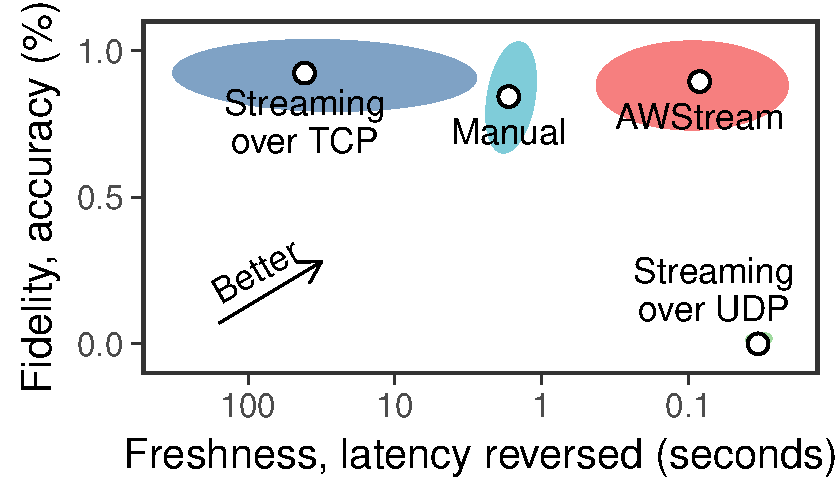
\includegraphics[width=0.8\columnwidth]{figures/figure1.pdf}
  \caption{The trade-off space between data freshness and fidelity when facing
    insufficient bandwidth (details in \autoref{sec:runtime-adaptation}).}
  \label{fig:intro}
  \vspace{-1em}
\end{figure}

Applications that simply use existing protocols without any attempt at
adaptation can result in extreme design points. E.g., streaming over TCP ensures
reliable delivery (hence high fidelity) but backlogged data delays the delivery
of data (hence freshness suffers).  On the other hand, streaming over UDP
minimizes latency by sending packets as fast as possible, but uncontrolled
packet loss can devastate data fidelity.

Manual policies, such as sampling, allow developers to trade data fidelity for
freshness~\cite{rabkin2014aggregation}. However, it's difficult to write
accurate policies without extensive domain expertise or considerable effort. In
practice, developers write manual policies based on heuristics rather than
quantitative measurements and, as we show in \autoref{sec:evaluation}, such
policies can lead to sub-optimal performance in terms of both freshness and
fidelity.

Furthermore, application-specific optimizations often do not generalize. A
fine-tuned adaptation algorithm for one application works poorly for a different
application, if performance metrics or data distributions change.  For example,
video streaming focuses on quality of experience
(QoE)~\cite{michalos2012dynamic, pantos2016http, yin2015control}. Because humans
favor smoothness over image quality, these systems maintain a high frame rate,
e.g.\,\(25~\text{FPS}\), and reduce the resolution under bandwidth limitation.
However, low resolution images can lead to poor accuracy for video analytics
that rely on the image details, e.g.\,face detection~\cite{viola2001rapid}.

In this paper, we present \sysname{}, a framework for building adaptive stream
processing applications that simultaneously simplifies development \emph{and}
improves application accuracy in the face of limited or varying wide-area
bandwidth.
% for the wide area that achieves low latency and high accuracy simultaneously
% with minimal developer effort.
\sysname{} achieves this through the combination of three novel contributions:

\begin{enumerate}[leftmargin=*, topsep=3pt]
\item \sysname{} introduces new programming abstractions by which a developer
  expresses \emph{what} degradation functions can be used by the framework.
  % {\bf Sylvia: Cut remainder of para? Too much detail for intro?}  More
  % specifically, \sysname{} augments existing stream processing operators with
  % a new \maybe{} operator. Its basic form takes a function that degrades the
  % input stream, and a list of values that serve as a knob to control the level
  % of degradation.  and . The knob specifies the degradation level that affects
  % data size and data fidelity.  We extend the basic form with a library of
  % specialized operators for common data types, such as
  % \texttt{maybe\_downsample} for images.  Our API is \textit{composable}
  % (multiple operators form a configuration that affects the adaptation
  % jointly), and \textit{extensible} (arbitrary functions and external
  % libraries can be embedded with our operators).
  Importantly, developers do not have to specify exactly when and how different
  degradation functions are to be used which is instead left to the \sysname{}
  framework.

\item Rather than rely on manual policies, \sysname{} automatically
  \emph{learns} a Pareto-optimal policy or strategy for when and how to invoke
  different degradation functions.  For this, we design a methodology that uses
  a combination of offline and online training to build an accurate model of the
  relationship between an application's accuracy and its bandwidth consumption
  under different combinations of degradation functions. Our solution exploits
  parallelism and sampling-based techniques to efficiently explore the
  configuration space and learn an optimal strategy.

  % The key idea is to \textit{automatically} build an accurate and precise
  % \textit{performance model} instead of relying on manual policies or
  % application-specific optimizations.
  % We use an \textit{offline} process to bootstrap our system with
  % developer-supplied training data, and continuously refine the profile
  % \textit{online} to handle \textit{model drift}.  We exploit parallelism and
  % sampling-based techniques to efficiently explore the configuration space and
  % learn a adaptation strategy.

\item \sysname{}'s final contribution is the design and implementation of a
  runtime system that continually measures and adapts to network conditions.
  \sysname{} matches the streaming data rate to the measured available
  bandwidth, and achieves high accuracy by using the learned Pareto-optimal
  configurations.  Upon encountering network congestion, our adaptation
  algorithm increases the degradation level to reduce the data rate, such that
  no persistent queue builds up. To recover, it progressively decreases the
  degradation level after probing for more available bandwidth.

  % The runtime also provides additional options to control application
  % behaviors, such as limiting the maximum
  % allowed WAN bandwidth. For multiple applications, the profiles can be used
  % to allocate bandwidth among competing tasks for \textit{utility fairness}.
\end{enumerate}

We implement \sysname{} and use it to prototype three streaming applications:
augmented reality (AR), pedestrian detection (PD), and distributed Top-K
(TK). We use real-world data to profile these applications and evaluate their
runtime performance on a geo-distributed public cloud.  We show that
\sysname{}'s data-driven approach generates accurate profiles and that our
parallelism and sampling techniques can speed up profiling by up to 29$\times$
and 8.7$\times$\@ respectively.

We show that \sysname{} significantly outperforms non-adaptive applications:
e.g., achieving a more than 100$\times$ reduction in packet delivery times
relative to applications built over TCP, or an over 88\% improvement in data
fidelity (application accuracy) relative to applications built over UDP.  We
also compare \sysname{} to JetStream~\cite{rabkin2014aggregation}, a
state-of-the-art system for building adaptive streaming analytics that is based
on manual policies: our results show that besides the benefit of generating
optimal policies \textit{automatically}, \sysname{} achieves a 15-20$\times$
reduction in latency and 1-5\% improvement in accuracy relative to JetStream. We
show that these gains come from the combination of \sysname{}'s ability to learn
better policies \emph{and} its well-designed runtime.  Hence, the ease of
development that \sysname{} provides comes with significantly \emph{improved}
application performance compared to typical manually crafted policies.

%%% Local Variables:
%%% mode: latex
%%% TeX-master: "../awstream"
%%% End:

\section{Motivation}
\label{sec:motivation}

In this section, we first examine the gap between high application demands and
limited WAN bandwidth. We then show that neither manual policies nor
application-specific optimizations solve the problem.

\subsection{Wide-area Streaming Applications}
\label{sec:wide-area-streaming}

We focus on wide-area streaming analytics, especially the emerging IoT
applications. We give two concrete examples.

\para{Video Surveillance.} We envisage a city-wide monitoring system that
aggregates camera feeds, from stationary ground cameras and moving aerial
vehicles, and analyzes video streams in real time for surveillance, anomaly
detection, or business intelligence~\cite{oh2011large}. Recent advances in
computer vision have dramatically increased the accuracy for automatic visual
scene analysis, such as pedestrian detection~\cite{dollar2012pedestrian},
vehicle tracking~\cite{coifman1998real}, and facial recognition to locate people
of interest~\cite{Lu:2015:SHF:2888116.2888245, parkhi2015deep}. While some
surveillance cameras use dedicated links, an increasing number of surveillance
systems, such as Dropcam~\cite{dropcam} and Vigil~\cite{zhang2015design}, use
the public Internet and wireless links to reduce the cost of deployment and
management.

% \para{High-frequency IoT Sensors:} Although environmental sensors used to be
% slow and not data-intensive~\cite{atzori2010internet}, increasingly,
% high-frequency, high-precision sensors are deployed. For example, uPMUs
% monitor the electrical grid with a network of 1000 devices; each produces 12
% streams of 120 Hz high-precision values accurate to 100 ns. This amounts to
% 1.4 million points per second~\cite{andersen2016btrdb}.

\para{Infrastructure Monitoring.} Large organizations today are managing tens of
datacenters and edge clusters worldwide~\cite{calder2013mapping}. This
geo-distributed infrastructure continuously produces large volumes of data such
as data access logs, server monitoring logs, and performance
counters~\cite{alspaugh2014analyzing, pu2015low, vulimiri2015global}. While most
log analysis today runs in a batch mode on a daily basis, there is a trend
towards analyzing logs in real time for rapid
optimization~\cite{rabkin2014aggregation}. For example, CDNs can improve the
overall efficiency by optimizing data placement if the access logs can be
processed in real time. In Industrial IoT, large-scale real-time sensor
monitoring is becoming pervasive to detect anomalies, direct controls, and
predict maintenance ~\cite{balani2016enterprise, ge}.

%% ~\cite{xu2009detecting} We generated the HDFS logs by setting up a Hadoop
%% cluster on 203 EC2 nodes and running sample Hadoop map-reduce jobs for 48
%% hours, generating and processing over 200 TB of random data. We collected
%% over 24 million lines of logs from HDFS.

% We consider the practical issues with deploying these applications in the
% wide-area. Our stand is that these applications face a bigger network
% challenge.  Data generated from the edge often fail to be delivered to the
% processing site because of the scarce and variable bandwidth capacity in the
% wide-area. Once they arrive, existing stream processing systems can easily
% manage a large cluster and perform data analytics at real-time.

\subsection{Wide-area Bandwidth Characteristics}
\label{sec:wide-area-bandwidth}

WAN bandwidth is insufficient and costly, as shown by other
systems~\cite{hsieh17gaia, pu2015low, vulimiri2015wananlytics,
  vulimiri2015global}. Using Amazon EC2 as a case study, the WAN bandwidth
capacity is 15x smaller than their LAN bandwidth on average, and up to 60x
smaller in the worst case~\cite{hsieh17gaia}. In terms of pricing, the average
WAN bandwidth cost is up to 38x of the cost of renting two
machines~\cite{amazon2017pricing, hsieh17gaia}.

In addition to the scarcity and cost, the large variability of WAN bandwidth
also affects streaming workloads. We conducted a day-long measurement with
iPerf~\cite{iperf3} to study the pair-wise bandwidth between four Amazon EC2
sites (N. California, N. Virginia, Tokyo, Ireland).  The results show large
variance in almost all pairs---\autoref{fig:bw} is one such pair. There are
occasions when the available bandwidth is below 25\% of the maximum bandwidth.

\begin{figure}
  \centering
  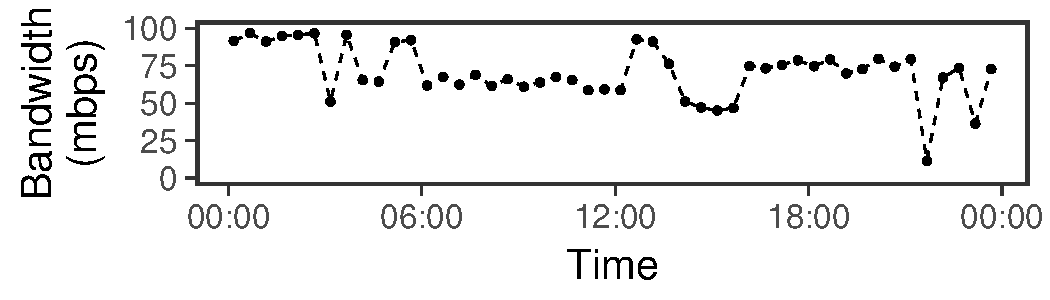
\includegraphics[width=0.9\linewidth]{figures/aws-variation.pdf}
  \caption{Bandwidth variations throughout the day between Amazon EC2 sites
    (from Ireland to California).}
  \label{fig:bw}
\end{figure}

The back-haul links between EC2 sites are better---if not at least
representative---in comparison to general WAN links. Similar scarcity and
variations exist in wireless networks~\cite{biswas2015large}, broadband access
networks~\cite{grover2013peeking, sundaresan2014bismark} and cellular
networks~\cite{nikravesh2014mobile}.

\subsection{Motivation for \sysname{}}
\label{subsec:motivation}

\pgfplotstableread[row sep=\\,col sep=&]{
  Frame Rate & Bandwidth (normalized) & Accuracy \\
  30 & 100 & 100 \\
  10 & 40 & 92 \\
  5 & 21 & 90 \\
  3 & 13 & 87 \\
  2 & 9 & 84 \\
}\stationaryframerate
\pgfplotstableread[row sep=\\,col sep=&]{
  Resolution & Bandwidth (normalized) & Accuracy \\
  1080p & 100 & 100 \\
  900p & 79 & 87 \\
  720p & 54 & 84 \\
  540p & 29 & 71 \\
  360p & 17 & 11 \\
}\stationaryresolution

\pgfplotstableread[row sep=\\,col sep=&]{
  Frame Rate & Bandwidth (normalized) & Accuracy \\
  30 & 100 & 100 \\
  10 & 65 & 64 \\
  5 & 46 & 32 \\
  3 & 34 & 18 \\
  2 & 27 & 10 \\
}\mobileframerate
\pgfplotstableread[row sep=\\,col sep=&]{
  Resolution & Bandwidth (normalized) & Accuracy \\
  1080p & 100 & 100 \\
  900p & 69 & 99 \\
  720p & 49 & 97 \\
  540p & 33 & 93 \\
  360p & 22 & 87 \\
}\mobileresolution

\captionsetup[subfigure]{
  font=scriptsize,
  justification=centering
}

\pgfplotsset{
  my bar/.style={%
    ybar,
    xtick pos=left,
    ytick pos=left,
    bar width               = .24cm,
    width                   = 1.2\textwidth,
    height                  = 0.124\textheight,
    xtick                   = data,
    enlarge x limits        = 0.15,
    nodes near coords,
    every node near coord/.append style={font=\tiny},
    nodes near coords align = {vertical},
    ymin                    = 0,
    ymax                    = 130,
    xlabel                  = {},
  }
}

\begin{figure*}
  \begin{minipage}{0.65\textwidth}
    \centering
    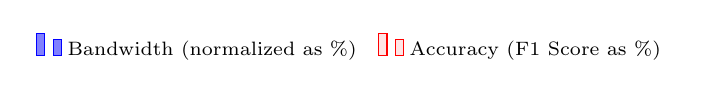
\begin{tikzpicture}
      \tikzstyle{every node}=[font=\scriptsize]
      \begin{axis}[
        width = 4cm,
        height = 2cm,
        hide axis,
        xmin=0,
        xmax=1,
        ymin=0,
        ymax=1,
        legend style={
          draw = none,
          legend columns= -1},
          /tikz/every even column/.append style={column sep=0.2cm},
        ]
        \addlegendimage{ybar, ybar legend, blue, fill=blue!50!white}\addlegendentry{B}
        \addlegendimage{ybar, ybar legend, red, fill=red!10!white}\addlegendentry{A}
        \legend{Bandwidth (normalized as \%), Accuracy (F1 Score as \%)}
      \end{axis}
    \end{tikzpicture}
  \end{minipage}
  \hfill
  \begin{minipage}{0.2\textwidth}
  \end{minipage}
  \\
  \vspace{0.1em}

  %%%
  %% First Half
  %%%

  \begin{subfigure}{0.07\textwidth}
    \footnotesize
    \centering
    \vspace{-2em}
    Stationary \\
    Camera
  \end{subfigure}%
  \begin{subfigure}{0.24\textwidth}
    \begin{tikzpicture}
      \tikzstyle{every node}=[font=\scriptsize]
      \begin{axis}[my bar,
        symbolic x coords = {30, 10, 5, 3, 2},
        ]

        \addplot [draw=blue, fill=blue!50!white, text=blue]
        table[x = Frame Rate, y = Bandwidth (normalized)]{\stationaryframerate};

        \addplot [draw=red, fill=red!10!white, text=red]
        table[x = Frame Rate, y = Accuracy]{\stationaryframerate};
        \legend{}
      \end{axis}
    \end{tikzpicture}
    \caption{Frame Rate \\ (resolution = 1080p)}
    \label{fig:stationary-frame-rate}
  \end{subfigure}%
  \begin{subfigure}{0.24\textwidth}
    \begin{tikzpicture}
      \tikzstyle{every node}=[font=\scriptsize]
      \begin{axis}[my bar,
        symbolic x coords = {1080p, 900p, 720p, 540p, 360p},
        ]
        \addplot [draw=blue, fill=blue!50!white, text=blue]
        table[x = Resolution, y = Bandwidth (normalized)]{\stationaryresolution};

        \addplot [draw=red, fill=red!10!white, text=red]
        table[x = Resolution, y = Accuracy]{\stationaryresolution};
        \legend{}
      \end{axis}
    \end{tikzpicture}
    \caption{Resolution \\ (frame rate = 30)}
    \label{fig:stationary-resolution}
  \end{subfigure}%
  \hspace{1em}
  \begin{subfigure}{0.2\textwidth}
    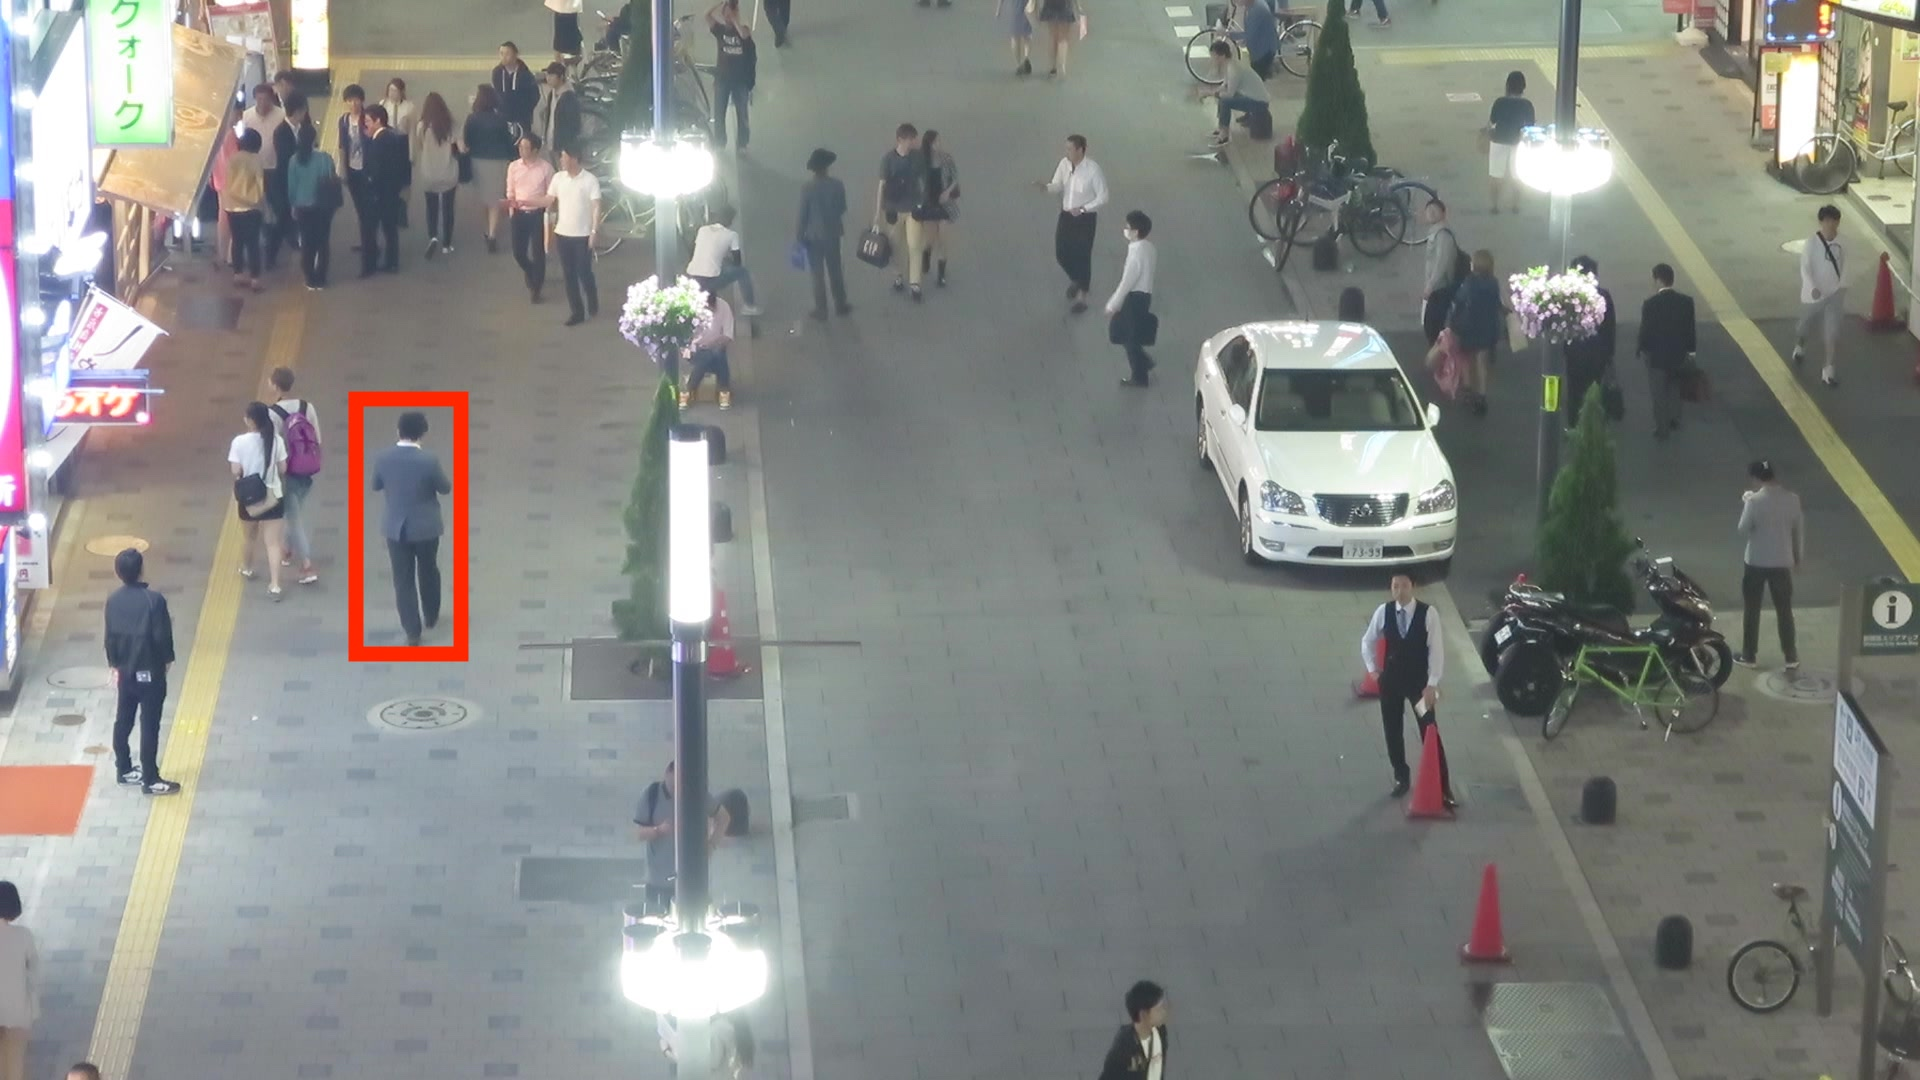
\includegraphics[width=\textwidth]{figures/mot-1.jpg}
    \caption{t=0s \\ small targets in far-field views}
  \end{subfigure}
  \hspace{.2em}
  \begin{subfigure}{0.2\textwidth}
    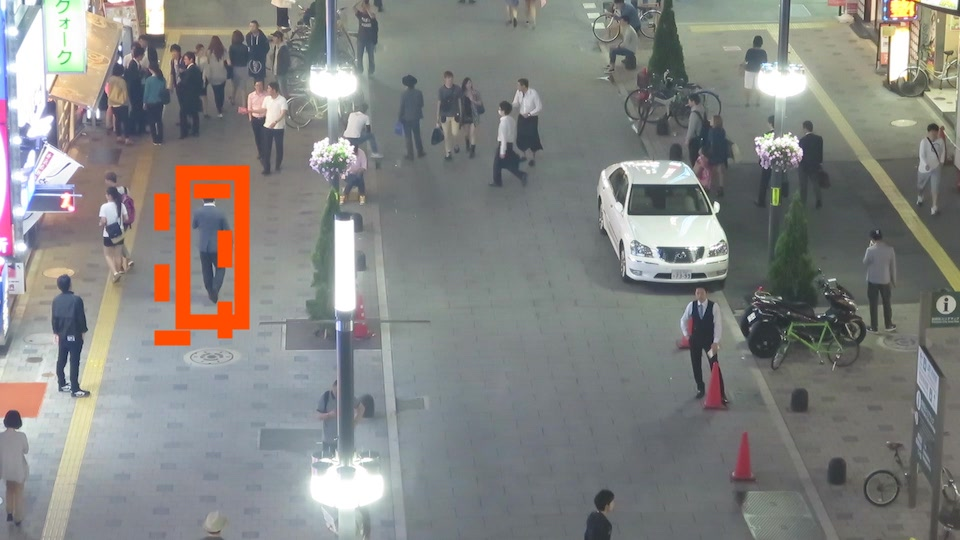
\includegraphics[width=\textwidth]{figures/mot-2.jpg}
    \caption{t=1s \\ small difference compared to t=0s}
  \end{subfigure}

  \vspace{0.7em}

  %%%%%%%%%%%%%%%%%%%%%%%%%%%%%%%%%%%%%%%%
  %% Second half
  %%%%%%%%%%%%%%%%%%%%%%%%%%%%%%%%%%%%%%%%

  \begin{subfigure}{0.07\textwidth}
    \footnotesize
    \centering
    \vspace{-3em}
    Mobile \\
    Camera
  \end{subfigure}%
  \begin{subfigure}{0.24\textwidth}
    \begin{tikzpicture}
      \tikzstyle{every node}=[font=\scriptsize]
      \begin{axis}[my bar,
        symbolic x coords = {30, 10, 5, 3, 2},
        ]
        \addplot [draw=blue, fill=blue!50!white, text=blue]
        table[x = Frame Rate, y = Bandwidth (normalized)]{\mobileframerate};

        \addplot [draw=red, fill=red!10!white, text=red]
        table[x = Frame Rate, y = Accuracy]{\mobileframerate};
        \legend{}
      \end{axis}
    \end{tikzpicture}
    \caption{Frame Rate \\ (resolution = 1080p)}
    \label{fig:mobile-frame-rate}
  \end{subfigure}%
  \begin{subfigure}{0.24\textwidth}
    \begin{tikzpicture}
      \tikzstyle{every node}=[font=\scriptsize]
      \begin{axis}[my bar,
        symbolic x coords = {1080p, 900p, 720p, 540p, 360p},
        ]
        \addplot [draw=blue, fill=blue!50!white, text=blue]
        table[x = Resolution, y = Bandwidth (normalized)]{\mobileresolution};

        \addplot [draw=red, fill=red!10!white, text=red]
        table[x = Resolution, y = Accuracy]{\mobileresolution};
        \legend{}
      \end{axis}
    \end{tikzpicture}
    \caption{Resolution \\ (frame rate = 30)}
    \label{fig:mobile-resolution}
  \end{subfigure}%
  \hspace{1em}
  \begin{subfigure}{0.2\textwidth}
    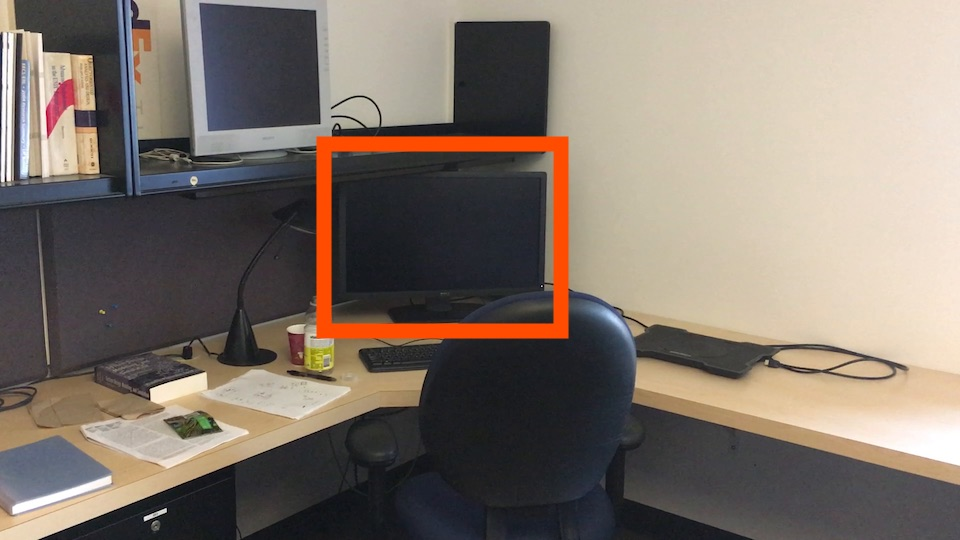
\includegraphics[width=\textwidth]{figures/darknet-1.jpg}
    \caption{t = 0s \\ nearby and large targets}
  \end{subfigure}
  \hspace{.2em}
  \begin{subfigure}{0.2\textwidth}
    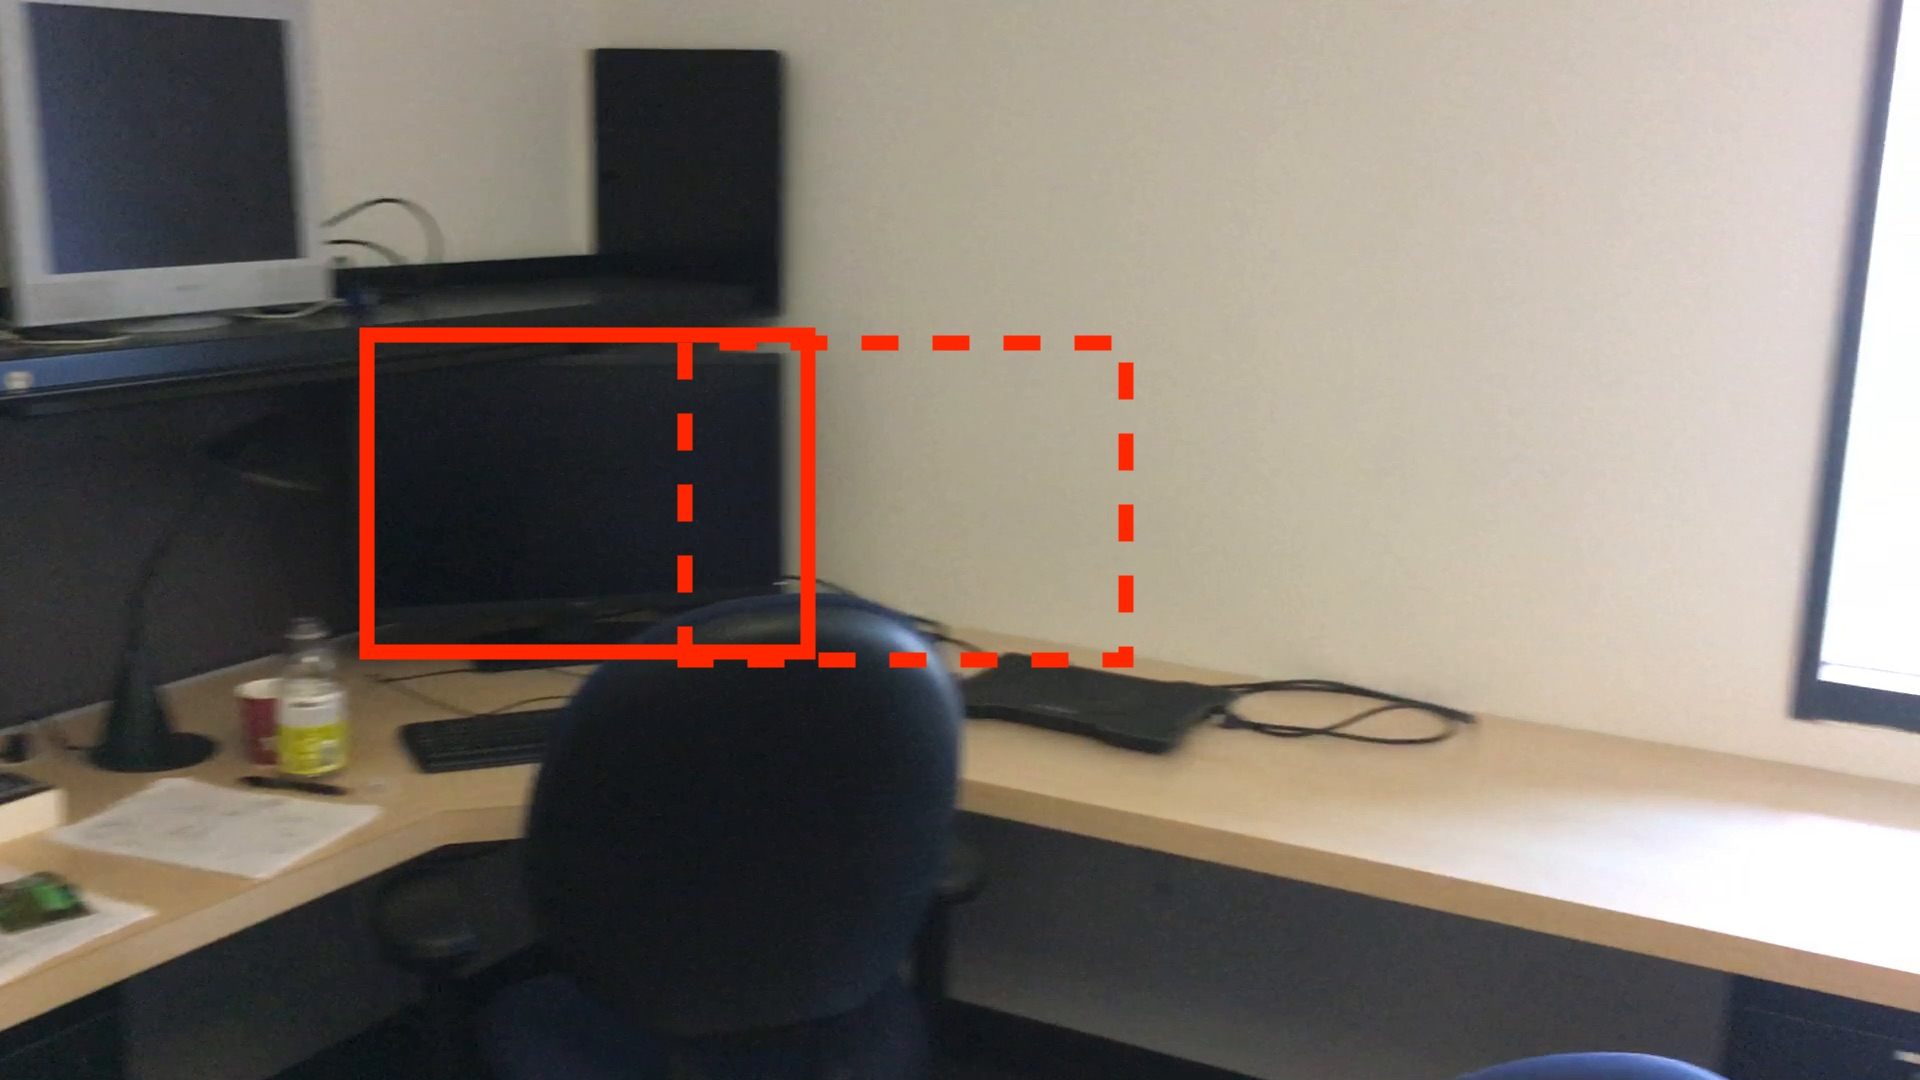
\includegraphics[width=\textwidth]{figures/darknet-2.jpg}
    \caption{t = 1s \\ large difference compared to t=0s}
  \end{subfigure}

  \caption{\cameraready{Redrawn}. The measured bandwidth and application accuracy for two video
    analytics applications. (1) Manual policies lack precision without
    measurements and need to handle multiple dimensions, as in (a-b) and
    (c-d). (2) Application-specific optimizations do not generalize: degrading
    frame rates works well for stationary camera (a), but not for mobile camera
    (e). (c-d) and (g-h) show example frames.}
  \label{fig:app-specific}
\end{figure*}

\captionsetup[subfigure]{
  font=small,
  skip=5pt,
}

%%% Local Variables:
%%% mode: latex
%%% TeX-master: "../awstream"
%%% End:


% \begin{figure*}
%   \centering
%   \includegraphics[width=0.85\linewidth]{figures/motiv-app-specific.pdf}
%   \caption{The measured bandwidth and application accuracy for two video
%     analytics applications. (1) Manual policies lack precision without
%     measurements and need to handle multiple dimensions (as in a-d). (2)
%     Application-specific optimizations do not generalize: degrading frame rates
%     works well for stationary camera (a), but not for mobile camera (c). (e-h)
%     shows example frames.}
%   \label{fig:app-specific}
% \end{figure*}

To address bandwidth limits, existing solutions use manual policies or
application-specific solutions. We discuss their drawbacks to motivate
\sysname{} (design in \autoref{sec:system}).

\para{Manual polices are sub-optimal.} JetStream~\cite{rabkin2014aggregation} is
the first to use degradation to address bandwidth limits in wide area. While
effective in comparison to non-adaptive systems, JetStream requires developers
to write manual policies, for example, ~\textit{``if bandwidth is insufficient,
  switch to sending images at 75\% fidelity, then 50\% if there still isn't
  enough bandwidth. Beyond that point, reduce the frame rate, but keep the image
  fidelity.''}\footnote{Excerpt from JetStream \S
  4.3~\cite{rabkin2014aggregation}.} We discuss the problems with manual
policies below and present quantitative evaluations in
\autoref{sec:runtime-adaptation}.

First, this policy is not accurate.  Developers write such rules based on
heuristics and do not back them up with measurements. Images with 75\% fidelity
do not necessarily lead to 75\% application accuracy. In terms of bandwidth,
naively one would think that reducing the frame rate by half will also half the
data rate. But if video encoding such as H.264~\cite{richardson2011h} is used, a
reduction in frame rate increases the inter-frame difference and creates
P-frames with larger sizes. \autoref{fig:mobile-frame-rate} shows that when
reducing the frame rate to 33\% (from \(30~\text{FPS}\) to \(10~\text{FPS}\)),
the bandwidth use can still be more than 50\%.

Second, it is not scalable to specify rules one by one. A fine-grain control
requires many rules in the policy. Besides, applications can degrade in multiple
dimensions and each dimension has different impacts (compare
\autoref{fig:stationary-frame-rate} with \autoref{fig:stationary-resolution}).
Specifying rules in detail and across dimensions manually is a tedious and
error-prone process.

Lastly, this abstraction is too low-level. It forces developers to study and
measure the impact of individual operations, prohibiting its wide adoption in
practice.

\para{Application-specific optimizations do not generalize.} Because each
application has different performance metrics and relies on different features,
a fine-tuned policy for one application will often work poorly for another. For
example, DASH~\cite{sodagar2011mpeg} optimizes QoE for video streaming; it keeps
a high frame rate and reduces resolutions for adaptation. Its policy that lowers
the resolution works poorly for video analytics that relies on image
details~\cite{lowe2004distinctive, viola2001rapid}. In
\autoref{fig:stationary-resolution}, we show that pedestrian detection accuracy
drops fast when reducing resolutions as pedestrian are small in the scenes.

Similar applications face different data distributions, as shown in
\autoref{fig:app-specific} between stationary cameras detecting pedestrians (up)
and mobile cameras recognizing objects (bottom). For stationary cameras, when we
consider the slow walking speed of pedestrians, a high frame rate is not
necessary. But high-resolution images are crucial because these surveillance
cameras are far away from the targets. In the mobile camera case, because the
camera moves, reducing the frame rate introduces significant errors.

%%% Local Variables:
%%% mode: latex
%%% TeX-master: "../awstream"
%%% End:

%% LocalWords: Dropcam IoT DCs geo CDNs iPerf JetStream scalable
%% LocalWords: bw runtime QoE analytics datacenters

\section{\sysname{} Design}
\label{sec:system}

\sysname{} avoids the problems with manual policies or application-specific
optimizations by structuring adaptation as a set of approximate, modular and
extensible specifications (\autoref{sec:struct-adapt}). The well-defined
structure allows us to build a generic profiling tool that learns an accurate
relationship, the profile, between bandwidth consumption and application
accuracy (\autoref{sec:automatic-profiling}). The profile then guides the
runtime to react with precision: achieving low latency and high accuracy when
facing bandwidth limitations (\autoref{sec:runtime}). \autoref{fig:overview}
shows the high-level overview of \sysname{}.

\begin{figure}
  \centering
  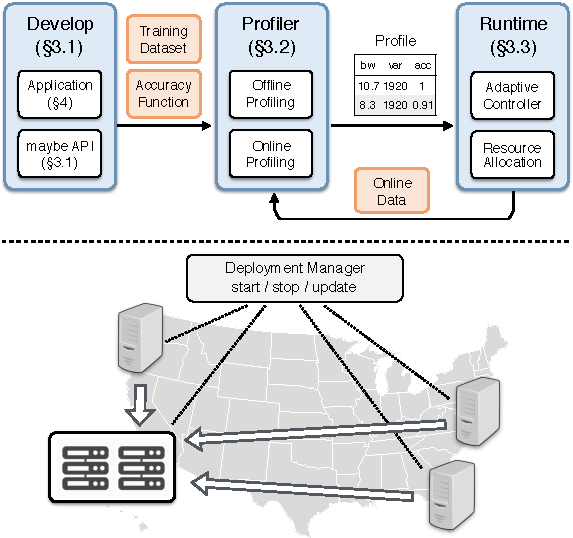
\includegraphics[width=0.8\linewidth]{figures/system.pdf}
  \caption{\sysname{}'s three phases: development, profiling and runtime.
    \sysname{} also manages wide-area deployment.}
  \label{fig:overview}
  \vspace{-1em}
\end{figure}

\subsection{API for Structured Adaptation}
\label{sec:structure-adapt}

%% Introduce graphs of operators model
Most stream processing systems construct applications as a directed graph of
operators~\cite{toshniwal2014storm, zaharia2013discretized}. Each operator
transforms input streams into new streams. \sysname{} borrows the same
computation model.  \autoref{tab:operators} lists some example operators, such
as \texttt{map} and \texttt{skip}.

To integrate adaptation as a first-class abstraction, \sysname{} introduces
\maybe{} operators that degrade data quality, yielding potential bandwidth
savings.  Our API design has three considerations. $(i)$~To free developers from
specifying exact rules, the API should allow specifications with
options. $(ii)$~To allow combining multiple dimensions, the API should be
modular: each operator is a unit and the developer can chain multiple
operators. $(iii)$~To support flexible integration with arbitrary degradation
functions, the API should take user-defined functions (UDFs). Therefore, our API
is,

\vspace{-2pt}
\begin{lstlisting}
        maybe(knobs: Vec<T>, f: (T, I) => I)
\end{lstlisting}

We illustrate the use of the \texttt{maybe} operator with an example that
quantizes a stream of integers in Rust:

\begin{table*}
  \small
  \centering
  \begin{tabular}{ c r l }
    \toprule
    \multirow{4}{*}{Normal Operators}
    & \textit{map} (f: I $\Rightarrow$ O) & Stream<I> $\Rightarrow$ Stream<O> \\
    & \textit{skip} (i: Integer) & Stream<I> $\Rightarrow$
                                   Stream<I> \\
    & \textit{sliding\_window} (count: Integer, f: Vec<I> $\Rightarrow$ O) & Stream<I> $\Rightarrow$
                                                                            Stream<O> \\
    % & \textit{tumbling\_window} (count: Integer, f: Vec<I> $\Rightarrow$ O) & Stream<I> $\Rightarrow$
    %                                                                          Stream<O> \\
    % & \textit{timed\_window} (time: Duration, f: Vec<I> $\Rightarrow$ O) & Stream<I> $\Rightarrow$
    %                                                                      Stream<O> \\
    & ... & ... \\
    \midrule
    \multirow{5}{*}{Degradation Operators}
    & \textit{maybe} (knobs: Vec<T>, f:  (T, I) $\Rightarrow$ I) & Stream<I> $\Rightarrow$
                                                                 Stream<I> \\
    & \textit{maybe\_skip} (knobs: Vec<Integer>) & Stream<I> $\Rightarrow$ Stream<I> \\
    & \textit{maybe\_head} (knobs: Vec<Integer>) & Stream<Vec<I>{}> $\Rightarrow$
                                                   Stream<Vec<I>{}> \\
    & \textit{maybe\_downsample} (knobs: Vec<(Integer, Integer)>) & Stream<Image> $\Rightarrow$ Stream<Image> \\
    & ... & ... \\
    \bottomrule
  \end{tabular}
  \vspace{0.2em}
  \caption{Stream processing operators in \sysname{}. \texttt{Vec<T>} represents
    a list of elements with type \texttt{T}.}
  \label{tab:operators}
  \vspace{-1em}
\end{table*}

\vspace{-2pt}
\begin{lstlisting}
let quantized_stream = vec![1, 2, 3, 4].into_stream()
    .maybe(vec![2, 4], |k, val| val.wrapping_div(k))
    .collect();
\end{lstlisting}

The snippet creates a stream of integers, chains a degradation operation, and
collects the execution result. In this example, the knob is [2, 4] and the
degradation function performs a wrapping (modular) division where the divisor is
the chosen knob. The knob value modifies the quantization level, affecting the
output: [1, 2, 3, 4] (no degradation), [0, 1, 1, 2] (k=2), or [0, 0, 0, 1]
(k=4). If the stream is then encoded---e.g. run-length encoding as in
JPEG~\cite{wallace1992jpeg}---for transmission, the data size will depend on the
level of degradation.

Based on the \texttt{maybe} primitive, one can implement additional degradation
operators for common data types. For instance, \texttt{maybe\_head} will
optionally take the top values of a list; \texttt{maybe\_downsample} can resize
the image to a configured resolution. \sysname{} provides a number of such
operations as a library to simplify application development
(\autoref{tab:operators}).

With our API, the example mentioned in \autoref{subsec:motivation} can now be
implemented as follows:

\vspace{-2pt}
\begin{lstlisting}
let app = Camera::new((1920, 1080), 30)
    .maybe_downsample(vec![(1600, 900), (1280, 720)])
    .maybe_skip(vec![2, 5])
    .map(|frame| frame.show())
    .compose();
\end{lstlisting}

This snippet first instantiates a \texttt{Camera} source, which produces
\texttt{Stream<Image>} with 1920x1080 resolution and 30 FPS\@. Two degradation
operations follow the source: one that downsamples the image to either 1600x900
or 1280x720 resolution, and the other that skips frames with a parameter of 2 or
5, resulting in 30/(2+1)=10 FPS or 30/(5+1)= 6 FPS\@. This example then shows
degraded images on the display. In practice, operators for further processing,
such as encoding and transmission, can be chained.

%%% Local Variables:
%%% mode: latex
%%% TeX-master: "../awstream"
%%% End:

%% LocalWords: UDFs Vec quantization quantized quantizes
%% LocalWords: downsample downsamples subsec

\subsection{Automatic Profiling}
\label{sec:automatic-profiling}

After developers use \maybe{} operators to specify potential degradation
operations, \sysname{} automatically builds an accurate profile. The profile
captures the relationship between \textit{application accuracy} and \textit{bandwidth
consumption}
under different \textit{combinations} of data degradation operations. We describe the
formalism, followed by techniques that efficiently perform offline and online
profiling.

\para{Profiling formalism.} Suppose a stream processing application has $n$
\maybe{} operators. Each operator introduces a knob $k_i$ and their combination
forms a \textit{configuration} $c = [k_{1}, k_{2}, ... k_{n}]$. The set of all
possible configurations $\mathbb{C}$ is the space that the profiling
explores. For each configuration $c$, there are two mappings that are of
particular interest: a mapping from $c$ to its bandwidth consumption $B(c)$ and
its accuracy measure $A(c)$. \autoref{tab:notations} summarizes the notations
used in this paper.

The profiling looks Pareto-optimal configurations, that is, for any
configuration $c$ in the Pareto-optimal set, there is no alternative
configuration $c'$ that requires less bandwidth and offers a higher
accuracy. The Pareto-optimal set $\mathbb{P}$ is defined mathematically as
follows:

{\small \vspace{-1em}
  \begin{equation}
  \mathbb{P} = \{ c \in \mathbb{C} : \{ c' \in \mathbb{C}: B(c') < B(c),
  A(c') > A(c) \} = \varnothing\}
  \label{eq:pareto}
\end{equation}
}%

\begin{table}
  \footnotesize
  \centering
  \begin{tabular}{r l}
    \toprule
    \textbf{Symbol} & \textbf{Description} \\
    \midrule
    $n$ & number of degradation operations \\
    $k_i$ & the \textit{i}-th degradation knob \\
    $c = [k_{1}, k_{2}, ... k_{n}]$ & one specific configuration \\
    $\mathbb{C}$ & the set of all configurations \\
    \midrule
    $B(c)$ & bandwidth requirement for $c$ \\
    $A(c)$ & accuracy measure for $c$ \\
    $\mathbb{P}$ & Pareto-optimal set \\
    \midrule
    $c_i$, $c_{i+1}$, $c_{\max}$ & current/next/maximal configuration at runtime \\
    $R$ & network delivery rate (estimated bandwidth) \\
    $\text{Q}_\text{E}$, $\text{Q}_\text{C}$ & messages when \texttt{Queue} is empty or congested \\
    $\text{R}_\text{C}$ & message when \texttt{Receiver} detects congestion \\
    $\text{AC}_\text{Probe}$ & message when \texttt{AC} requests probing \\
    $\text{S}_\text{ProbeDone}$ & message when \texttt{Socket} finishes probing \\
    \bottomrule
  \end{tabular}
  \caption{Notations used in this paper.}
  \label{tab:notations}
\end{table}

Because \sysname{} allows arbitrary functions as the degradation functions, it
does not assume a closed-form relation for $B(c)$ and $A(c)$. Instead,
\sysname{} takes a data-driven approach: profiling applications with
developer-supplied training data.  We measure $B(c)$ at the point of
\textit{transmission}. The accuracy $A(c)$ is measured either against the \textit{ground-truth},
or the reference results when \textit{all degradation operations are off}.  We show
examples of concrete knobs, configurations, accuracy functions when we present
applications in \autoref{tab:apps}.

\para{Offline Profiling.} We first use an offline process to build a bootstrap
profile (or default profile).  \sysname{} makes no assumptions on the
performance models, and thus evaluate all possible configurations.  While all
knobs form a combinatorial space, the offline profiling is only a one-time
process.  We exploits parallelism to reduce the profiling time.  Without any
\textit{a priori} knowledge, all configurations are assigned randomly to
available machines.

% \para{Offline Profiling.} We first use an offline process to build a bootstrap
% profile (or default profile).  Because \sysname{} supports arbitrary
% degradation operations, we need to evaluate all combinations of the
% configurations offline profiling is a one-time process, \sysname{} currently
% performs an exhaustive evaluation of all configurations in $\mathbb{C}$
% despite all knobs form a combinatorial space. Future work could explore
% statistical methods to build performance models with a smaller number of
% training samples~\cite{venkataraman2016ernest, alipourfard2017cherrypick}.
% \sysname{} exploits parallelism when profiling all configurations.  Without
% any \textit{a priori} knowledge, all configurations are assigned randomly to
% all available machines.

\para{Online Profiling:} \sysname{} runs an online profiling process
continuously to refine the profile. The refinement handles \textit{model
  drifts}, a problem when the learned profile fails to predict the performance
accurately. There are two challenges with online profiling.  $(i)$~There is no
ground-truth labels or reference data to compute accuracy. Because labelling
data is prohibitively labor intensive and time
consuming~\cite{russell2008labelme}, \sysname{} currently uses \textit{raw data as
the
reference}. At runtime, if the application streams raw data, the data is used for
online profiling. Otherwise, we allocate additional bandwidth to back-haul raw
data, but only do so when there is spare capacity. $(ii)$~Exhaustive profiling
is expensive. If the profiling takes too much time, the newly-learned profile
may already be stale. \sysname{} uses a combination of parallelism and sampling
techniques to speed up this process, as below:

\begin{itemize}[leftmargin=*, topsep=0pt, itemsep=0pt]

\item Parallelization with degradation-aware scheduling. Evaluating each
  configuration takes a different amount of time. Typically, an increase in the
  level of degradation leads to a decrease in computation; for example, a
  smaller FPS means fewer images to process. Therefore, we collect processing
  times for each configuration from the offline process and schedule online
  profiling with longest first schedule (LFS)~\cite{karger2010scheduling} during
  parallelization.

\item Sampling-based profiling. Online profiling can speed up if we only profile
  a subset of all data or a subset of all configurations.  Sampling data reduces
  the amount of data to process, but at a cost of generating less accurate
  profiles. When sampling configuration, we can evaluate a subset of the
  Pareto-optimal configurations and compare their performances with the existing
  profile. A substantial difference, such as more than 1 mbps of bandwidth
  estimation, triggers a full profiling over all configurations to update the
  current profile.

\end{itemize}

%%% Local Variables:
%%% mode: latex
%%% TeX-master: "awstream"
%%% End:

\subsection{Runtime Adaptation}
\label{sec:runtime}

At runtime, \sysname{} matches data rate to available bandwidth to minimize
latency and uses Pareto-optimal configurations to maximize accuracy.

\begin{figure}
  \centering
  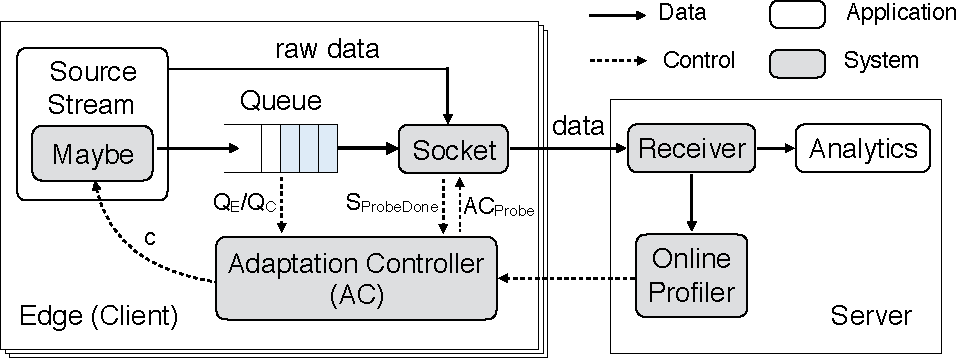
\includegraphics[width=\linewidth]{figures/runtime-adaptation.pdf}
  \caption{Runtime adaptation system architecture.}
  \label{fig:runtime}
\end{figure}

\autoref{fig:runtime} shows our runtime system architecture. \sysname{}
applications' source contains a \texttt{Maybe} module derived from all \maybe{}
operators. This module allows the controller to update the level of
degradation. Data generated by the source is then enqueued to \texttt{Queue} and
subsequently dequeued by \texttt{Socket}, which sends data over the network
using TCP. When the data generation rate exceeds \texttt{Socket}'s departure
rate, the queue grows. In this case, the adaptation controller (AC) queries the
estimated bandwidth from \texttt{Socket} and regulates the source stream by
updating the configuration. After the data is sent through the network,
\texttt{Receiver} delivers data to the application analytics. \texttt{Receiver}
also performs congestion detection and extracts raw data, if it presents.  It
tracks minimal latency (similar to how BBR tracks
\texttt{RTprop}~\cite{cardwell2017bbr} within a filter window) and reports
sudden latency spikes to clients as congestion signalling. Raw data is only
transmitted when the queue is empty and online profiling is enabled. After a new
profile is learned by the online profiler, it is fed back to AC for subsequent
adaptation.

\begin{figure}
  \begin{subfigure}[t]{\columnwidth}
    \centering
    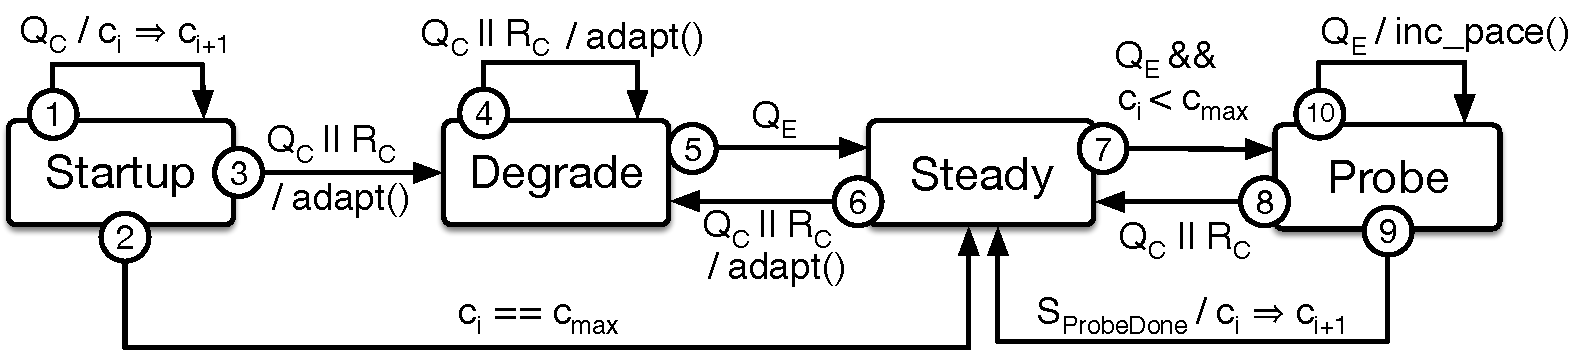
\includegraphics[width=\columnwidth]{figures/cc.pdf}
    \caption{Rate adaptation as a state machine.}
    \vspace{1em}
    \label{fig:cc-sm}
  \end{subfigure}
  \\
  \centering
  \begin{subfigure}[t]{\columnwidth}
    \centering
    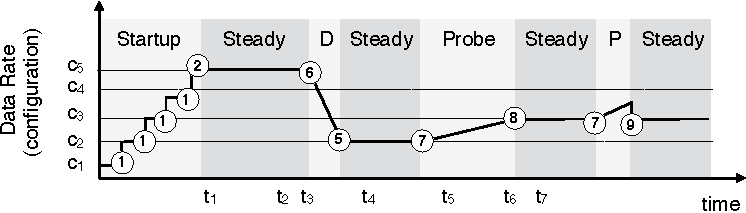
\includegraphics[width=0.9\columnwidth]{figures/cc2.pdf}
    \caption{An example illustrating the adaptation algorithm.}
    \label{fig:cc-ex}
  \end{subfigure}
  \caption{Runtime adaptation algorithm.}
  \label{fig:cc}
\end{figure}

\autoref{fig:cc-sm} shows the adaptation algorithm with a state machine model
and \autoref{fig:cc-ex} shows the state transitions with an example. AC loads
the profile and sorts all configurations with an ascending order of bandwidth
demand, resulting in a list $[c_1, \dots, c_{\max}]$.  These configurations
follow a total order: $c_i < c_j$ if $B(c_i) < B(c_j)$.  We denote the current
configuration as $c_i$ and the next $c_{i+1}$.  AC receives messages from the
\texttt{Queue}: message \qe{} when the queue is empty and $\text{Q}_\text{C}$
when queued items exceed a threshold. AC can query \texttt{Socket} for delivery
rate $R$ (arrow not shown) or request the source to probe
($\text{AC}_{\text{Probe}}$) for a target bandwidth, often $B(c_{i+1})$. If
there is no queue built up during the probing and $R > B(c_{i+1})$,
\texttt{Socket} sends back \spd{}. The reactions in each state are as follows:

\begin{itemize}[leftmargin=*, topsep=3pt, itemsep=0pt]

\item \textbf{Startup: rapid growth.} \sysname{} starts with $c_1$ and grows the
  rate ($c_i \Rightarrow c_{i+1}$) upon each \qe{}. The growth stops at
  $c_{\max}$ (to \texttt{Steady}) or if it receives \qc{}/\rc{} (to
  \texttt{Degrade}).

\item \textbf{Degrade: reacting to congestion.} Congestion is detected in two
  ways: (1) when \texttt{Queue} grows and exceeds a threshold, AC receives
  \qc{}; (2) when \texttt{Receiver} detects latency spikes, AC receives
  \rc{}. During congestion, AC runs the \texttt{adapt()} procedure by updating
  \texttt{Maybe} with the maximum-allowed $c$ that satisfies $B(c) < \alpha R$,
  where $\alpha \in (0, 1)$ and $R$ is \texttt{Socket}'s current delivery
  rate. A smaller $\alpha$ allows a quicker draining of the queue. After the
  congestion is resolved (\qe{} received), \sysname{} changes to
  \texttt{Steady}.

\item \textbf{Steady: low latency delivery.} \sysname{} achieves low latency by
  spending most of the time in the \texttt{Steady} state. It changes to
  \texttt{Degrade} when congestion occurs. If $c < c_{\max}$ and it receives
  \qe{}, AC enters the \texttt{Probe} state to check for more available
  bandwidth.

\item \textbf{Probe: more bandwidth for a higher accuracy.} Advancing the
  configuration directly causes a drastic latency increase when
  $B(c_{i+1}) \gg B(c_i)$. To allow a smooth increase, AC requests
  \texttt{Socket} to probe by sending additional traffic controlled by
  \texttt{probe\_gain} (in \texttt{inc\_pace()}, similar to
  BBR~\cite{cardwell2017bbr}). \sysname{} stops probing under two conditions:
  (1) upon \spd{}, it advances $c_i$; (2) upon \qc{} or \rc{}, it returns to
  \texttt{Steady}.

\end{itemize}

\subsection{Resource Allocation \& Fairness}

In addition to rate adaptation, the profile is also useful for controlling a
single application's bandwidth usage or allocating resources among competing
tasks.

For individual applications, developers can pin-point a configuration for a
given bandwidth or accuracy goal. They can also specify a criterion to limit
effective configurations. For example, \sysname{} can enforce an upper bound on
the bandwidth consumption. In this way, applications can control their bandwidth
costs while using the profile to maximize accuracy.

For multiple applications, their profiles allow novel bandwidth allocation
schemes such as utility fairness. Different from traditional resource fairness
with which applications get equal share of bandwidth, utility fairness aims to
maximize the \textit{minimal} application accuracy. With the profiles, bandwidth
allocation is equivalent to finding proper configuration $c^t$ for application
$t$. We formulate utility fairness as follows:

%% Pick one based on the space

\begin{equation}
 \label{eq:multitask}
 \underset{c^t}{\max} \; \min({A^t(c^t)})
 \;
 \text{s.t.}
 \;
 \sum_t{B^t(c^t)} < R
\end{equation}

% \begin{equation}
%  \label{eq:multitask}
%  \begin{aligned}
%     & \underset{c^t}{\text{maximize}} & & \min({A^t(c^t)}) & & \\
%     & \text{subject to} & & \sum_t{B^t(c^t)} < R & & \\
%  \end{aligned}
% \end{equation}

Solving this optimization is computationally hard. \sysname{} uses a heuristics
approach. It starts with $c^t_1$ and improves the application $t$ with the worst
accuracy. This process repeats until all available bandwidth is
allocated~\cite{zhang2017live}.

%%% Local Variables:
%%% mode: latex
%%% TeX-master: "../awstream"
%%% End:


%%% Local Variables:
%%% mode: latex
%%% TeX-master: "../awstream"
%%% End:

\section{Implementation}
\label{sec:implementation}

While our proposed API is general and not language specific, we have implemented
\sysname{} prototype in Rust (\textasciitilde 4000 lines of code). \sysname{} is
open source on GitHub.\footnote{URL elided for anonymity.}  Applications use
\sysname{} as a library and configure the execution mode---profiling, runtime as
client, or runtime as server---with command line arguments.

% \begin{figure}
%   \centering
%   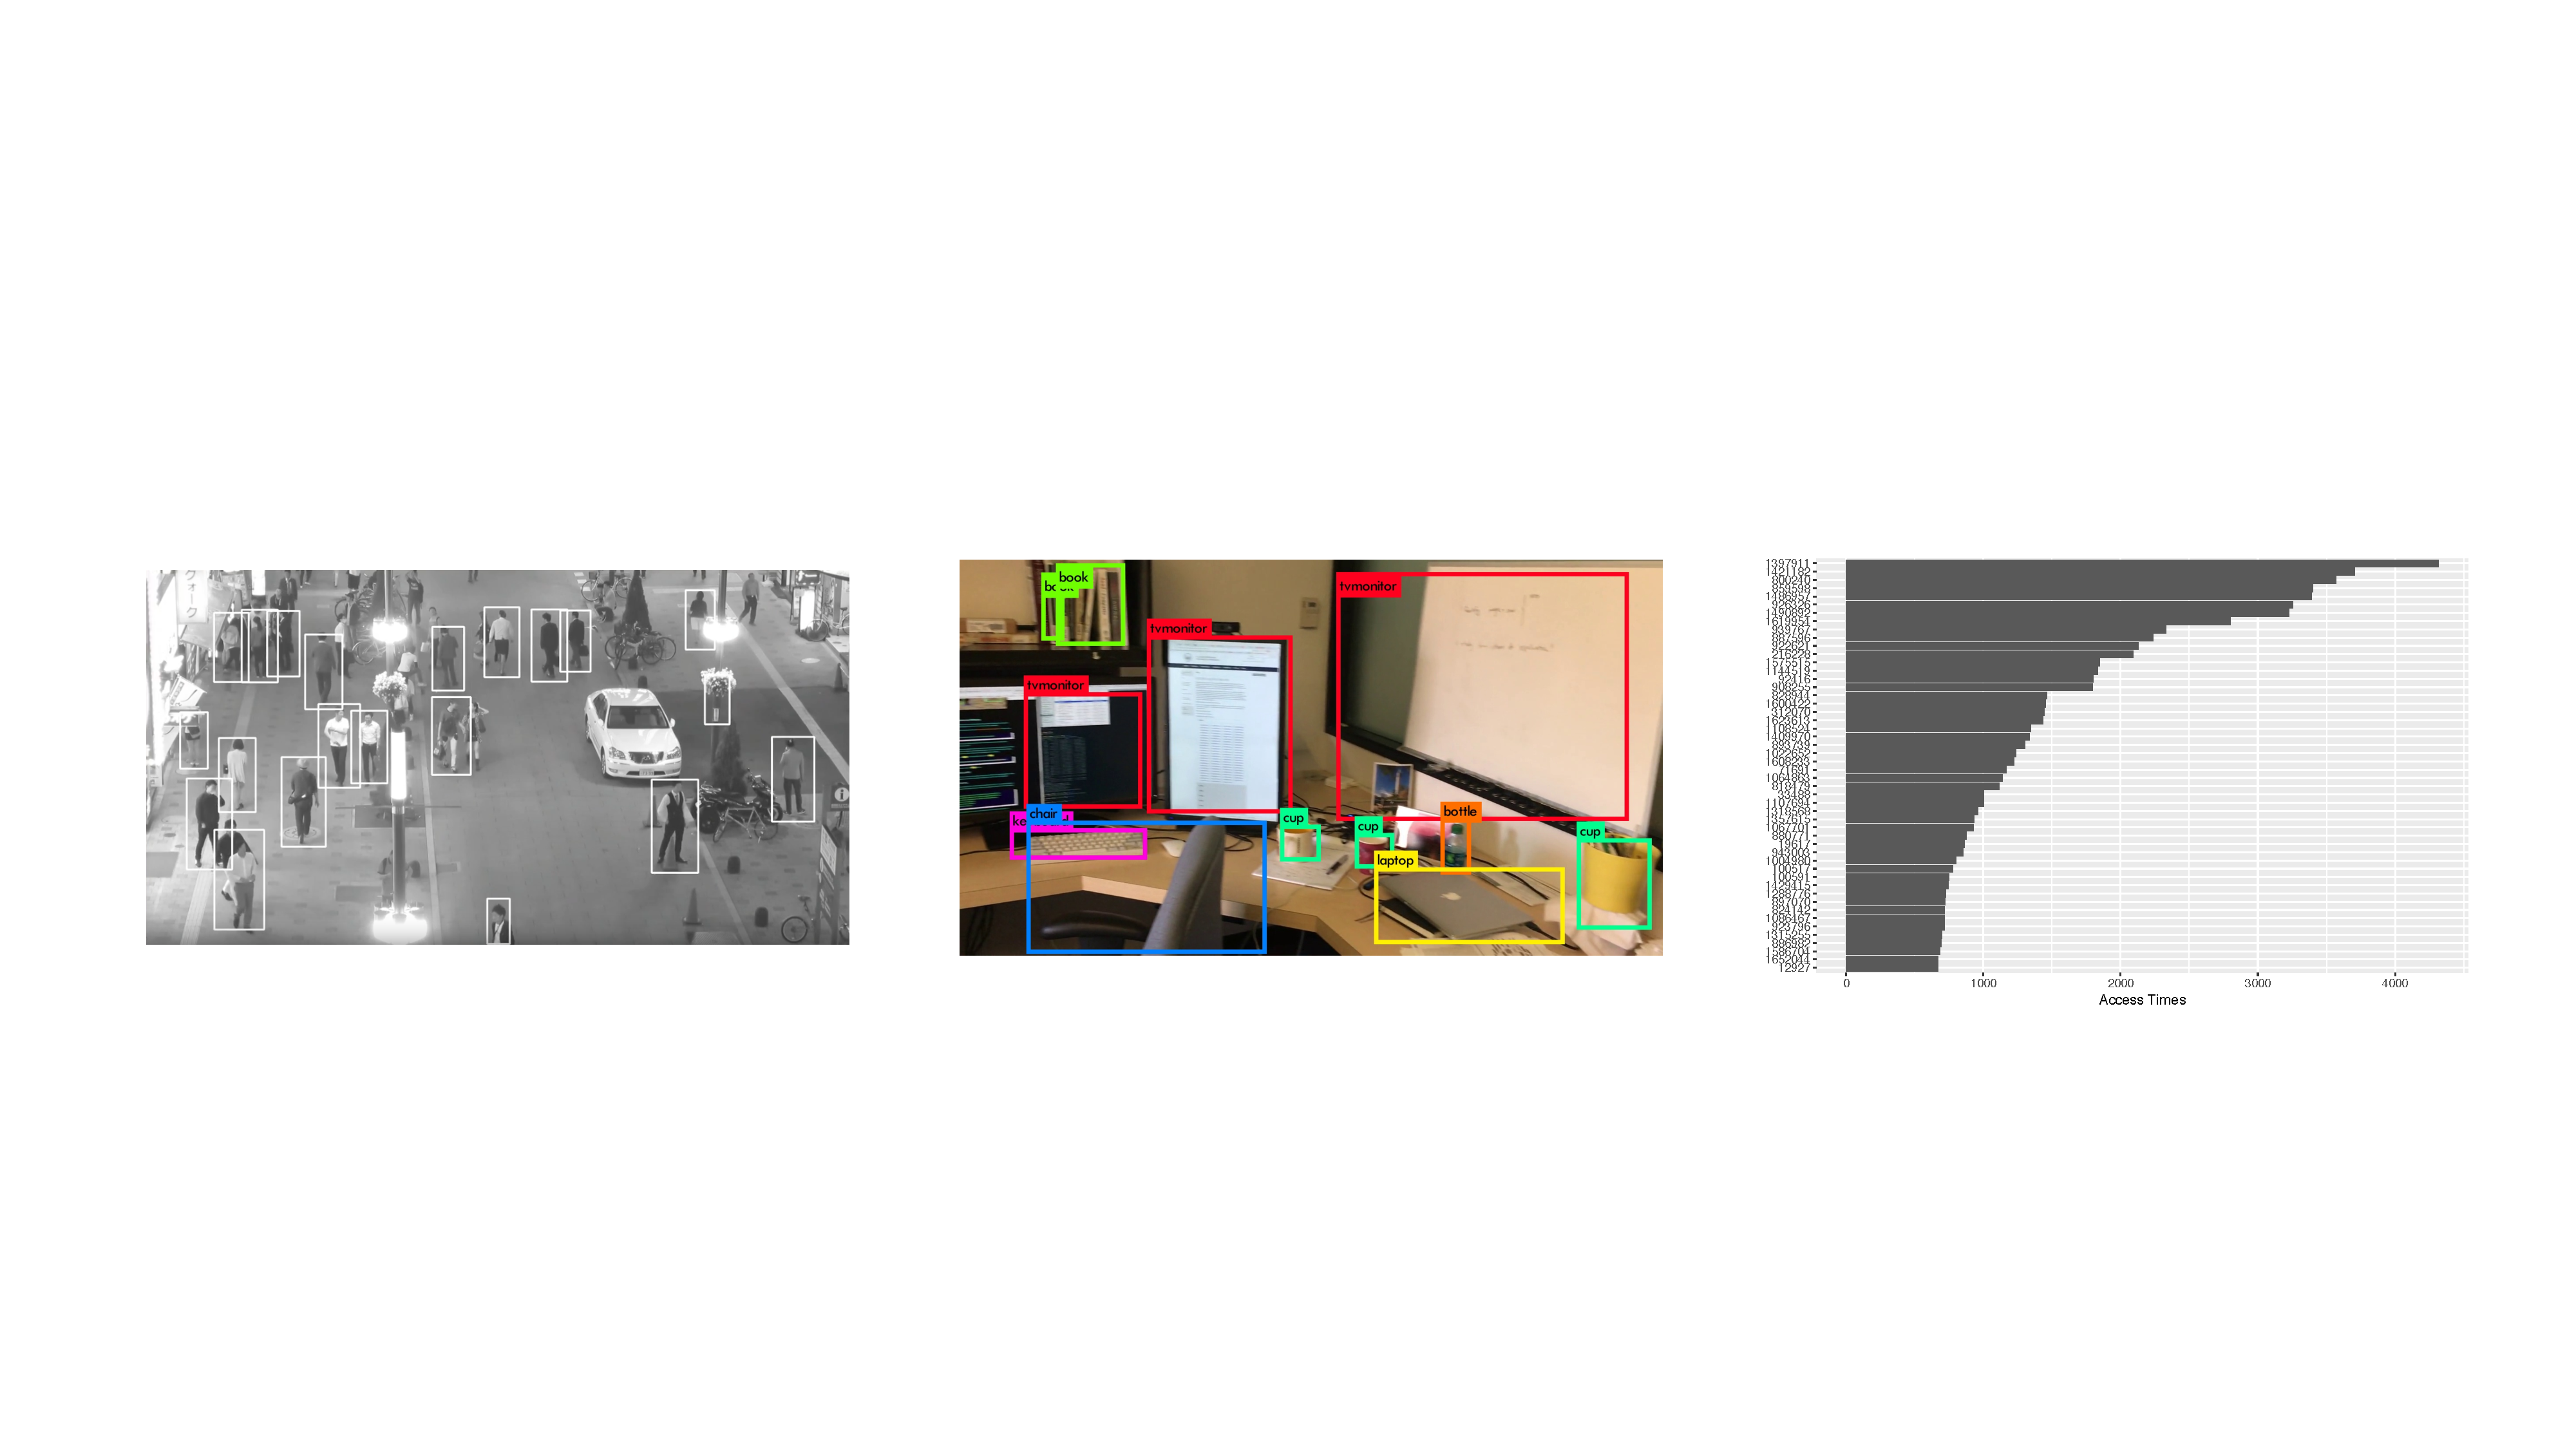
\includegraphics[width=\columnwidth]{figures/apps.pdf}
%   \caption{Three \sysname{} applications: augmented reality, pedestrian
%     detection, and distributed Top-K.}
%   \label{fig:three-apps}
% \end{figure}

\begin{table}
  \footnotesize
  \centering
  \begin{tabular}{c c c c}
    \toprule
    Application & Knobs & Accuracy & Dataset \\
    \midrule
    \specialcell{Augmented\\Reality}
                & \specialcell{resolution \\ frame rate \\ quantization }
                & F1 score~\cite{Rijsbergen:1979:IR:539927}
                & \specialcell{iPhone video clips\\training: office (24
    s)\\testing: home (246 s)} \\
    \midrule
    \specialcell{Pedestrian\\Detection}
                & \specialcell{resolution \\ frame rate \\ quantization }
                & F1 score
                & \specialcell{MOT16~\cite{milan2016mot16}\\training: MOT16-04\\testing: MOT16-03} \\
    \midrule
    \specialcell{Log Analysis\\(Top-K, K=50)}
                & \specialcell{head (N) \\ threshold (T) }
                & \specialcell{Kendall's $\tau$~\cite{abdi2007kendall}}
                & \specialcell{\href{https://www.sec.gov}{SEC.gov} logs~\cite{edgarlog} \\ training: 4 days \\
    testing: 16 days} \\
    \bottomrule
  \end{tabular}
  \vspace{0.5em}
  \caption{Application details.}
  \label{tab:apps}
  \vspace{-1em}
\end{table}

Using \sysname{}, we have built three applications: augmented reality (AR) that
recognizes nearby objects on mobile phones, pedestrian detection (PD) for
surveillance cameras, and a distributed log analysis to extract the Top-K mostly
accessed files (TK). \autoref{tab:apps} summarizes the application-specific
parts: knobs, accuracy functions, and datasets.

\para{Augmented Reality.} We target at augmented reality applications running on
mobile phones that recognize nearby objects by offloading the heavy computation
elsewhere, e.g.\,the cloud. Our implementation uses OpenCV
3.1~\cite{opencvlibrary} for image-related operations and YOLO~\cite{darknet13,
  redmon2016yolo9000}, a GPU-enabled pre-trained neural network, for object
recognition. Videos are encoded with H.264~\cite{richardson2011h}. Our
implementation uses GStreamer~\cite{gstreamer} with \texttt{x264enc} plugin
(\texttt{zerolatency} and constant quality). The quantization factor affecting
encoding quality becomes a knob in addition to image resolutions and frame
rates.

Object recognition returns a list of bounding boxes with the type of the
object. Each bounding box is a rectangle with normalized coordinates on the
image. We compare the detection against the reference result from raw data, and
declare it success if the intersection over union (IOU) is greater than
50\%~\cite{everingham2010pascal} and the object type matches. We use F1
score~\cite{Rijsbergen:1979:IR:539927} as the accuracy function. In terms of
dataset, we collected our own video clips: the training data is a 24-second long
video of an office environment; the test data is a 246-second long video of a
home environment.

\para{Pedestrian Detection.} This application analyzes streams of videos from
installed CCTV cameras and detects pedestrians inside. We use a similar setup
(OpenCV and GStreamer) as our augmented reality application except for the
analytical function. To detect pedestrians, we use GPU-accelerated histogram of
oriented gradients (HOG)~\cite{dalal2005histograms} with the default linear SVM
classifier from OpenCV. Because we do not recognize individual pedestrians, a
successful detection in this case only requires matching the bounding box. Our
evaluation uses MOT16 dataset~\cite{milan2016mot16} for both profiling and
runtime.

\begin{figure}
  \centering
  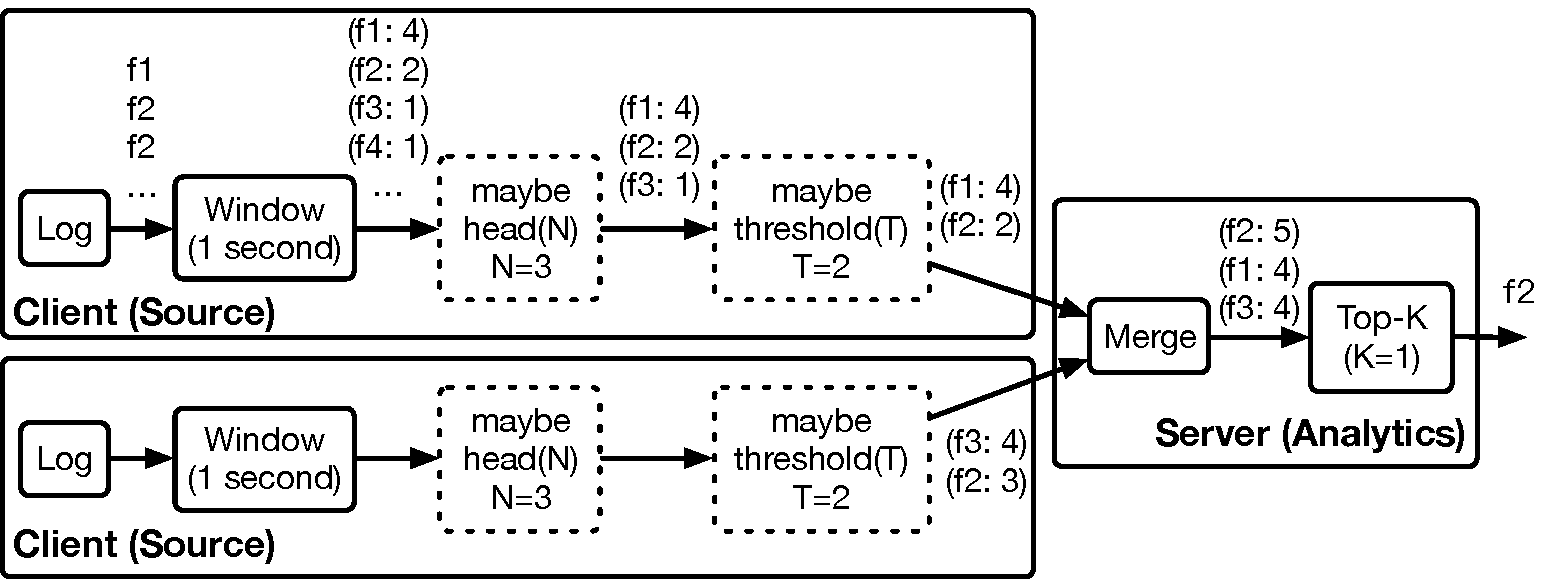
\includegraphics[width=\columnwidth]{figures/topk.pdf}
  \caption{A distributed Top-K application with two degradation operations:
    \texttt{head} and \texttt{threshold}. In this example, \texttt{f2}, which is
    not in Top-1 for either client, becomes the global Top-1 after the merge. It
    would have been purged if the clients use threshold T=3, demonstrating
    degradation that reduces data sizes affects fidelity.}
  \label{fig:topk}
  \vspace{-0.5em}
\end{figure}

\para{Distributed Top-K.} This application aggregates machine logs from
geo-distributed servers to find out the Top-K most accessed files, similar to
many Top-K queries~\cite{babcock2003distributed}. \autoref{fig:topk} illustrates
our processing pipeline with two degradation operations. First each source node
summarizes the log using \texttt{Window} operator to reduce the data size, a
pre-processing step. As many real-world access patterns follow a long tail
distribution, there is a large-but-irrelevant tail that contributes little to
the final Top-K. Each source node then filters the tail: (1) head(\texttt{N})
takes the top \texttt{N} entries; (2) threshold(\texttt{T}) filters small
entries whose count is smaller than \texttt{T}. These two operations affect the
final result and the exact impact depends on data distribution. We implement
these two operators by using \sysname{}'s \maybe{} abstraction.

To measure the accuracy, we need to compare the correlation between two ranked
list. Kendall's~$\tau$~\cite{abdi2007kendall} is a correlation measure of the
concordance between two ranked list. The output ranges from \(-1\) to 1,
representing no agreement to complete agreement. To integrate with \sysname{},
we convert Kendall's~$\tau$ to [0, 1] with a linear transformation. For our
evaluation, we set K as 50 and use Apache log files that record and store user
access statistics for the \href{https://www.sec.gov}{SEC.gov} website. The logs
are split into four groups, simulating four geo-distributed nodes monitoring web
accesses. To match the load of popular web servers, we compress one hour's logs
into one second.

%%% Local Variables:
%%% mode: latex
%%% TeX-master: "../awstream"
%%% End:

\begin{figure*}[htb]
  \centering
  \begin{subfigure}[t]{0.32\textwidth}
    \centering
    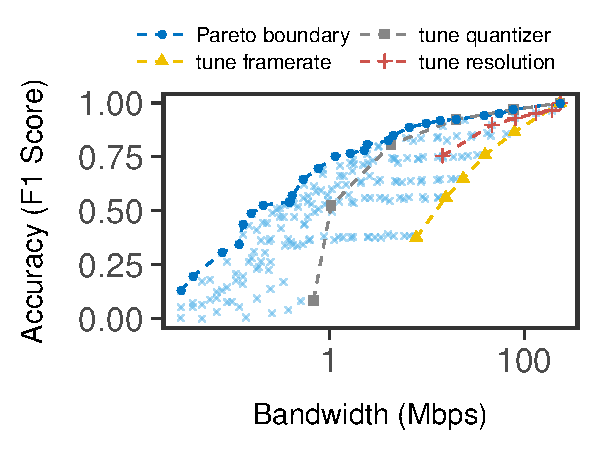
\includegraphics[width=\textwidth]{figures/profile-darknet.pdf}
    \caption{Augmented Reality (AR)}
    \label{fig:ar-profile}
  \end{subfigure}
  \hfill
  \begin{subfigure}[t]{0.32\textwidth}
    \centering
    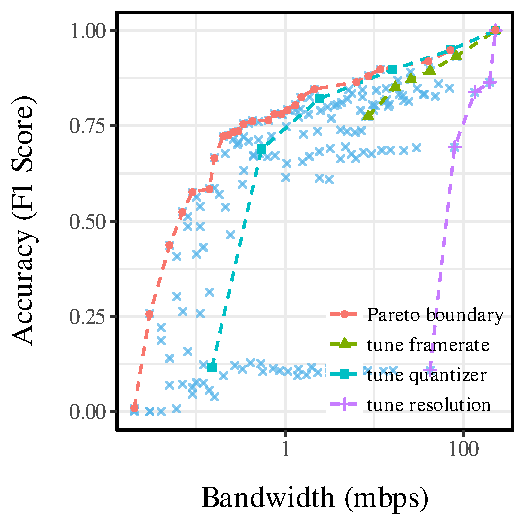
\includegraphics[width=\textwidth]{figures/profile-mot.pdf}
    \caption{Pedestrian Detection (PD)}
    \label{fig:pd-profile}
  \end{subfigure}
  \hfill
  \begin{subfigure}[t]{0.32\textwidth}
    \centering
    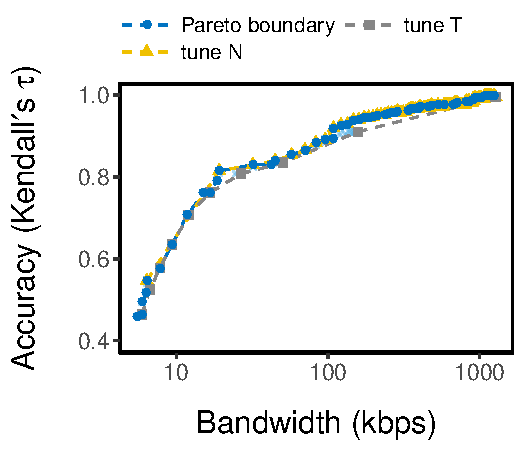
\includegraphics[width=\textwidth]{figures/profile-topk.pdf}
    \caption{Top-K (TK)}
    \label{fig:tk-profile}
  \end{subfigure}
  \caption{Application profiles of three applications. Each cross point is one
    configuration $c$'s performance $(B(c), A(c))$. All figures show the Pareto
    boundary as well as the performance if only tuning one dimension. Note the
    x-axis is in log scale.}
  \label{fig:all-profiles}
  \vspace{-0.5em}
\end{figure*}

\section{Evaluation}
\label{sec:evaluation}

In this section, we show the evaluations of \sysname{}, summarizing the results
as follows.

\begin{itemize}[itemsep=0pt, topsep=3pt]
\item[\autoref{sec:application-profiles}] \sysname{} generates Pareto-optimal
  profiles across multiple dimensions with precision
  (\autoref{fig:all-profiles}).
\item[\autoref{sec:online-profiling}] Our parallel and sampling techniques
  speeds up offline and online profiling (\autoref{fig:parallel},
  \autoref{fig:online-tricks}).
\item[\autoref{sec:runtime-adaptation}] At runtime, all \sysname{} applications
  achieve sub-second latency and nominal accuracy drop
  (\autoref{fig:ar-runtime}, \autoref{fig:pd-runtime},
  \autoref{fig:tk-runtime}).
\item[\autoref{sec:various-rtt}] \sysname{} maintains low latency performance
  across different network conditions (\autoref{fig:ar-rtt}).
\item[\autoref{sec:multi-task-alloc}] \sysname{} profiles allow different
  resource allocations: resource fairness and utility fairness
  (\autoref{fig:multitask}).
\end{itemize}

\subsection{Application Profiles}
\label{sec:application-profiles}

We run offline profiling using the training dataset described
in~\autoref{tab:apps} and show the learned profiles in
\autoref{fig:all-profiles}. In each figure, the cross dots represent the
bandwidth demand and application accuracy for one configuration. We highlight
the Pareto-optimal boundary $\mathbb{P}$ with blue dashed lines. To understand
each dimension's impact on the degradation, we highlight configurations from
tuning only \textit{one} dimension. From these profiles, we make the following
observations:

\para{Large bandwidth variation.} For all three applications, The bandwidth
requirements of all three applications have two to three orders of magnitude of
difference (note the x-axis is in log scale). For AR and PD, the most expensive
configuration transmits videos at 1920x1080, 30 FPS and 0 quantization; it
consumes \SI{230}{Mbps}. In contrast to the large bandwidth variation, there is
a smaller variation in accuracy. In PD, for example, even after the bandwidth
reduces to \SI{1}{Mbps} (less than 1\% of the maximum), the accuracy is still
above 75\%. The large variation allows \sysname{} to operate at a high accuracy
configuration even under severe network deterioration.

\para{Distinct effects by each dimension.} Comparing dashed lines in each
profile, we see that the Pareto-optimal configurations are only achievable when
multiple knobs are in effect. Tuning only one dimension often leads to
sub-optimal performance. Within a single profile, the difference between tuning
individual dimensions is evident. For PD, tuning resolution (the red line) leads
to a quicker accuracy drop than tuning frame rate (the yellow line). Comparing
AR and PD, the same dimension has different impact. Tuning resolution is less
harmful in AR than PD; while tuning frame rate hurts AR more than PD\@. This
echoes our initial observation in~\autoref{subsec:motivation} that
application-specific optimizations do not generalize.

% \para{Quantification with precision}. The generated profiles are actionable
% configurations that control the knobs with precision. For example, if PD
% transmits video at 1920x1080 resolution, \(10~\text{FPS}\) and a quantization
% of 20, it will consume 11.7 mbps of bandwidth, achieving roughly 90\%
% accuracy. This saves developers from laboriously analyzing their application
% to compute manual policies.

\subsection{Profiling Efficiency \& Online Profiling}
\label{sec:online-profiling}

This section focuses on the AR application as a case study; our profiling
techniques---parallelism and sampling---do not make assumptions about the
application; therefore, the evaluation results can be generalized to other
applications.

In AR, there are 216 different configurations: 6 resolutions, 6 frame rates and
6 quantization levels. AR uses YOLO~\cite{redmon2016yolo9000}, a neural network
model for object detection. It takes roughly \SI{30}{\ms} to process one frame
on GeForce\textregistered\space GTX 970.\footnote{YOLO resizes an input image to
  a fixed resolution (416x416) as required by the neural network. It takes a
  similar amount of time to Evaluating each image (with different resolutions).}
But different configurations require different times for processing. For
example, a \(10~\text{FPS}\) video has 1/3 of the frames to process in
comparison to a \(30~\text{FPS}\) video.  In our experiment, to evaluate all 216
configurations, it takes 52 seconds for 1 second worth of data. We denote such
overhead as 52X\@. \hyperref[sec:automatic-profiling]{Section 3.2} have
discussed parallel and sampling techniques to improve the profiling efficiency;
we present their evaluations as follows.

\begin{figure}
  \centering
  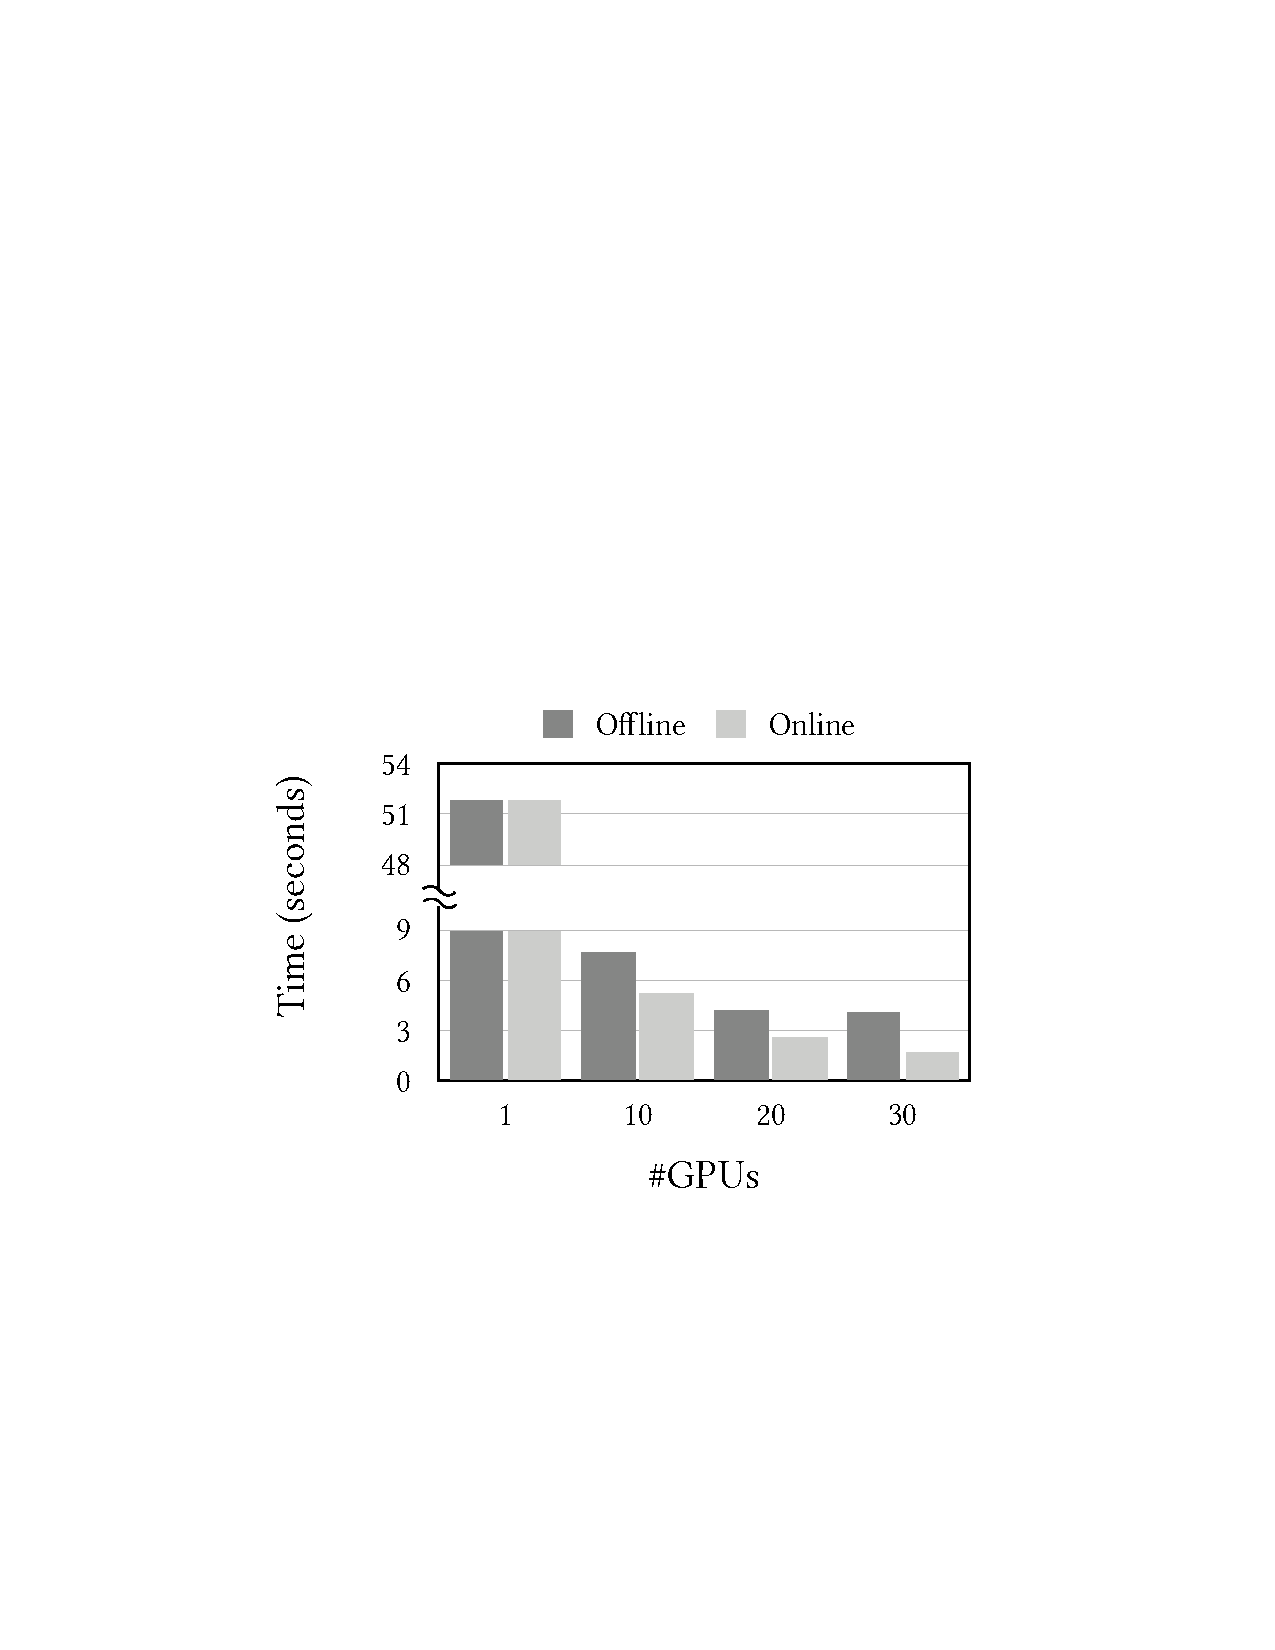
\includegraphics[width=1.0\columnwidth]{figures/parallel.pdf}
  \caption{Parallelism speeds up both offline and online profiling.
  The y-axis shows the profiling time for 1-second video.}
  \label{fig:parallel}
  \vspace{-0.5em}
\end{figure}

\para{Parallelism reduces the profiling time (\autoref{fig:parallel})}. Because
evaluating each individual configuration is independent of other configurations,
we parallelize the profiling task by assigning configurations to GPUs.
$(i)$~Our offline profiling assigns configurations randomly.  With the increased
number of GPUs, the overhead reduces from 52X to 4X with 30 GPUs.  $(ii)$~Our
online profiling assigns configurations based on the processing times collected
during offline.  \sysname{} uses LFS~\cite{karger2010scheduling} to minimize the
makespan and reduces the overhead to 1.75X with 30 GPUs (29$\times$ gain).

\para{Sampling techniques speed up online profiling
  (\autoref{fig:online-tricks}).}  Before we evaluate the speed up, we validate
\textit{model drift} with real-world data. We use the profile trained in an
office environment.  According to the profile, the application should operate at
a configuration of 1280x720, \SI{30}{FPS} and 20 quantization to meet an
\SI{11}{Mbps} goal.  We test it against a home environment, and at about t=100s,
the camera points out of the window to detect objects on the street. Because of
the scene change, the configuration fails to predict runtime bandwidth, as
illustrated in \autoref{fig:offline}.

To correct the profile, if we continuously run the profiling online and update
the profile, the application will choose the right configuration to meet the
bandwidth limit.  \autoref{fig:online} shows the bandwidth prediction when we
continuously profile with the past 30 seconds of video. At time t=120s, the new
prediction corrects the drift. The downside of continuous profiling, as
discussed earlier, is the cost: 52X overhead with 1 GPU\@. In addition to
parallelism, \sysname{} uses sampling techniques for online profiling
(improvements in \autoref{tab:online}):

(i) Partial data. Instead of using all the past data, we run profiling with only
a fraction of the raw data.  \autoref{fig:online-partial} shows the bandwidth
consumption if the profiling uses only 10 seconds of data out of the past 30
seconds. In this way, although the profile may be less accurate (the
mis-prediction at t=80-100s), and there is a delay in reacting to data change
(the mis-prediction is corrected after t=125s), we save the online profiling by
3$\times$ (from 52X to 17X).

(ii) Partial configurations. If we use the past profile as a reference and only
measure a subset of all Pareto-optimal configurations, the savings can be
substantial. A full profiling is only triggered if there is a significant
difference. \autoref{fig:online-trigger} shows the bandwidth prediction if we
evaluate 5 configurations continuously and trigger a full profiling when the
bandwidth estimation is off by \SI{1}{Mbps} or the accuracy is off by 10\%.  For
our test data, this scheme is enough to correct model drifts by predicting an
accurate bandwidth usage (compare \autoref{fig:online} and
\autoref{fig:online-trigger}).  The overhead reduces to 6X because we run full
profiling less often (only two full profiling). It is an 8.7$\times$ gain.

\begin{figure}
  \centering
  \begin{subfigure}[t]{0.45\columnwidth}
    \centering
    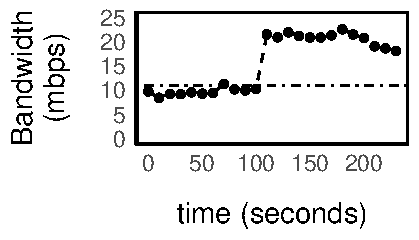
\includegraphics[width=\textwidth]{figures/online1.pdf}
    \caption{Offline only}
    \label{fig:offline}
  \end{subfigure}
  \hfill
  \begin{subfigure}[t]{0.45\columnwidth}
    \centering
    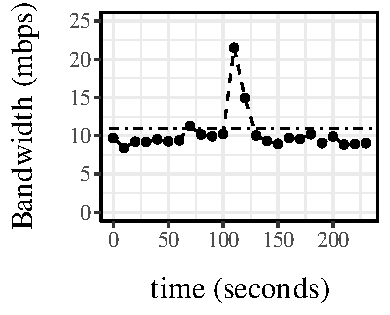
\includegraphics[width=\textwidth]{figures/online2.pdf}
    \caption{Online (continuous)}
    \label{fig:online}
  \end{subfigure}
  \\
  \vspace{0.5em}
  \begin{subfigure}[t]{0.45\columnwidth}
    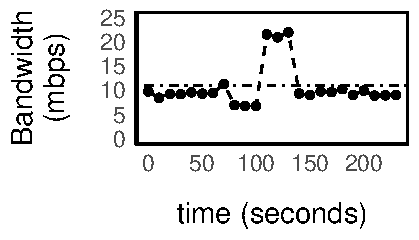
\includegraphics[width=\textwidth]{figures/online3.pdf}
    \caption{Partial data}
    \label{fig:online-partial}
  \end{subfigure}
  \hfill
  \begin{subfigure}[t]{0.45\columnwidth}
    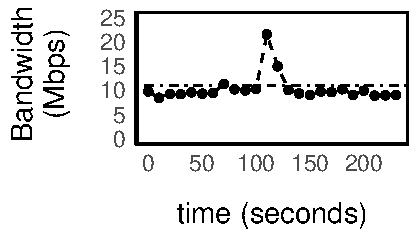
\includegraphics[width=\textwidth]{figures/online4.pdf}
    \caption{Partial configurations}
    \label{fig:online-trigger}
  \end{subfigure}
  \caption{The horizontal reference line is the target bandwidth
    (\SI{11}{Mbps}). (1) Online profiling is necessary to handle model drift
    ((a) vs.\,(b-d)). (2) Sampling techniques---partial data (c) and partial
    configurations (d)---can correct model drift with less profiling overhead
    (see \autoref{tab:online}), compared to continuous (b).  We omit accuracy
    predictions since in all schemes \sysname{} finds configurations that
    achieve similarly high accuracy (\textasciitilde 90\%).  }
  \label{fig:online-tricks}
  \vspace{-0.5em}
\end{figure}

%% Offline: 0
%% Online: 1 frame (1852.21 GPU * seconds)
%% Online (1/10)   (185.2 GPU * seconds)
%% Trigger         ( GPU * seconds)

\begin{table}[t]
  \small
  \centering
  \begin{tabular}{c c c}
    \toprule
    Online scheme & Overhead & Improvements \\
    \midrule
    Continuous & 52X & Baseline \\
    Partial data & 17X & 3$\times$\\
    Partial configurations & 6X & 8.7$\times$ \\
    \bottomrule
  \end{tabular}
  \caption{Compared to the continuous profiling baseline (52X overhead), our
    sampling techniques speed up by 3$\times$ or 8.7$\times$.}
  \label{tab:online}
  \vspace{-1em}
\end{table}

Note that these techniques---parallelization, sampling data, and sampling
configurations---can be combined together to further reduce the profiling
overhead. For example, scheduling five GPUs running 5 configurations
continuously to check for model drift will reduce the overhead to 1X\@. In
practice, the amount of resources to use depends on the budget and the
importance of the job. \sysname{} currently requires developers to configure the
application with proper online profiling techniques.

%% Note that it is not always needed to do online profiling. PD's test data
%% doesn't exhibit model drift.  Nor is online profiling always
%% expensive. Processing TK over all configurations.

\subsection{Runtime Adaptation}
\label{sec:runtime-adaptation}

In this section, we evaluate the runtime performance by controlling available
bandwidth across geo-distributed sites and compare \sysname{} with baselines
including streaming over TCP/UDP, JetStream, and video streaming. Our evaluation
shows that \sysname{} achieves low latency and high accuracy simultaneously
across all applications. We first discuss AR in depth and then present the
results of PD/TK.

\para{Experiment setup.} We conduct our experiments on four geo-distributed
machines from Amazon EC2, spanning four different regions. Three (at
N.\,Virginia, Ohio, Oregon) act as worker nodes and one (at N.\,California) acts
as the analytics server. The average RTTs from the workers to the server are
\SI{65.2}{\ms}, \SI{22.2}{\ms}, and \SI{50.3}{ms}.

During the experiment, each worker transmits test data (\autoref{tab:apps}) for
about 10 mins. If the duration of the test data is less than 10 mins, it
loops. Because $B(c_{\max})$ is prohibitively large (raw videos consumes
\SI{230}{Mbps} ), we use a reasonable configuration to limit the maximum
rate. In our AR experiment, $c_{\max}$ is 1600x900 resolution, \(30~\text{FPS}\)
and a quantization of 20; it consumes about \SI{14}{Mbps}.

Our bandwidth control scheme follows
JetStream~\cite{rabkin2014aggregation}. During the experiment, we use the Linux
\texttt{tc} utility with HTB~\cite{htb, lartc} to control the clients' outgoing
bandwidth. Each experiment involves four phases: $(i)$~before t=200s, there is
no shaping; $(ii)$~at t=200s, we limit the bandwidth to \SI{7.5}{Mbps} for 3
minutes; $(iii)$~at t=380s, we further decrease the available bandwidth to
\SI{5}{Mbps}; $(iv)$~ at t=440s, we remove all traffic shaping. For UDP, HTB
doesn't emulate the packet loss or out-of-order delivery; so we use
\texttt{netem} and configure the loss probability according to the delivery
rate. Because each pair-wise connection has a different capacity, we impose a
\textit{background} bandwidth limit---\SI{25}{Mbps}---to simplify comparisons.

We compare \sysname{} with the following baselines:

\begin{itemize}[noitemsep, nolistsep, leftmargin=*]

\item Streaming over TCP/UDP (non-adaptive). $(i)$~For TCP, we re-use
  \sysname{}'s runtime that runs over TCP but disable the adaptation. $(ii)$~For
  UDP, we use FFmpeg~\cite{bellard2012ffmpeg} to stream video:
  RTP/UDP~\cite{schulzrinne2006rtp} for media and RTSP for
  signaling~\cite{schulzrinne1998rtsp}. This is a common setup for video
  conferencing and IP cameras~\cite{durresi2005rtp, king2009cisco}.

\item Adaptive video streaming. We use HTTP Live Streaming (HLS) to represent
  popular adaptive video streaming techniques. Our setup resembles personalized
  live streaming systems~\cite{wang2016anatomy} but uses a smaller chunk for low
  latency (1 second instead of typical 2-10 seconds).\footnote{The appendix
    includes details about our HLS setup.}

\item JetStream with the manual policy described in \autoref{subsec:motivation}.

\item JetStream++, a modified version of JetStream that uses the profile learned
  by \sysname{}.\footnote{The appendix includes details about how we modified
    JetStream.}

\end{itemize}

At runtime, \sysname{} differs from JetStream in both policy and
adaptation. JetStream++ already improves over JetStream by using our
Pareto-optimal profile. \sysname{} improves the performance further with two
major changes: $(i)$~\sysname{} directly measures the delivery rate to select an
appropriate configuration to match available bandwidth while JetStream employs a
latency-based measure of capacity ratio. $(ii)$ \sysname{} has an explicit probe
phase while JetStream changes its policy immediately after capacity ratio
changes.

\begin{figure}[t]
  \begin{subfigure}[t]{\columnwidth}
    \centering
    \includegraphics[width=\columnwidth]{figures/runtime_darknet-timeseries.pdf}
    \caption{Time-series plot of the runtime behaviors: throughput (top),
      showing the effect of bandwidth shaping; latency (middle) in log scale;
      and accuracy (bottom).}
    \label{fig:ar-runtime-timeseries}
  \end{subfigure}
  \vspace{0.2em}
  \\
  \begin{subfigure}[t]{\columnwidth}
    \centering
    \includegraphics[width=\columnwidth]{figures/runtime_darknet-boxplot.pdf}
    \caption{Summary of latency and accuracy during the traffic shaping (between
      t=200s and t=440s).}
    \label{fig:ar-runtime-boxplot}
  \end{subfigure}
  \caption{For our AR application, \sysname{} simultaneously achieves low
    latency and high accuracy (with smaller variation).}
  \label{fig:ar-runtime}
  \vspace{-0.5em}
\end{figure}

\para{Results.} \autoref{fig:ar-runtime-timeseries} shows the runtime behavior
of \sysname{} and all baselines in time series. \autoref{fig:ar-runtime-boxplot}
summarizes the latency and accuracy with box plots during bandwidth shaping
(between t=200s and t=440s).

The throughput figure shows the effect of traffic shaping. During the shaping,
TCP and UDP make full use of the available bandwidth; in comparison, \sysname{},
JetStream, JetStream++, and HLS are conservative because of adaptation (see
their throughput drops). When we stop the shaping at t=440s, TCP has a
``catch-up'' phase when it is sending all queued items as fast as
possible. JetStream also has queued items because the policy in use (with only
three rules) cannot sustain \SI{5}{Mpbs} bandwidth. \sysname{} increases the
throughput gradually due to the explicit probing phase. HLS is the most
conservative scheme; it does not recover from degradation until t=500s.

 % summary(latency)
 %      Time        JetStream++        JetStream            HLS
 % Min.   :206.0   Min.   :  47.14   Min.   :  541.6   Min.   :3750
 % 1st Qu.:264.2   1st Qu.: 331.97   1st Qu.: 1544.6   1st Qu.:4960
 % Median :322.5   Median : 539.26   Median : 1732.1   Median :5438
 % Mean   :322.5   Mean   : 575.11   Mean   : 3105.8   Mean   :5578
 % 3rd Qu.:380.8   3rd Qu.: 771.06   3rd Qu.: 1951.0   3rd Qu.:6270
 % Max.   :439.0   Max.   :1599.51   Max.   :14245.7   Max.   :7085
 % Streaming over TCP Streaming over UDP    AWStream
 % Min.   :   290.8   Min.   :29.73      Min.   : 42.62
 % 1st Qu.: 28042.5   1st Qu.:31.51      1st Qu.: 50.59
 % Median : 54315.2   Median :33.18      Median : 79.51
 % Mean   : 55596.7   Mean   :33.08      Mean   :117.72
 % 3rd Qu.: 81514.5   3rd Qu.:34.90      3rd Qu.:156.22
 % Max.   :117780.4   Max.   :36.29      Max.   :648.08

The latency figures (both \autoref{fig:ar-runtime-timeseries} and
\autoref{fig:ar-runtime-boxplot}) show that \sysname{} is able to maintain
sub-second latency. During the traffic shaping, TCP queues items at the sender
side for up to hundreds of seconds. In contrast, UDP always transmits as fast as
possible, leading to a consistent low latency.\footnote{FFmpeg discards packets
  that miss a deadline (\SI{33}{\ms} for \SI{30}{FPS}).} HLS's latency
fluctuates around 4-5 seconds due to chunking, buffering, and network
variations, on par with recent literature~\cite{wang2016anatomy}. Both JetStream
and JetStream++ are able to adapt during traffic shaping. With a more precise
and fine-grain policy, JetStream++ achieves a lower latency (median
\SI{539}{\ms}) in comparison to JetStream (median \SI{1732}{\ms}). Because
JetStream's runtime reacts instantaneously when the congestion condition
changes, both baselines oscillate among polices during the
experiment. \sysname{} effectively addresses the oscillation with probing and
achieves a much lower latency (median \SI{118}{\ms}, 15$\times$ improvement over
JetStream and 5$\times$ improvement over JetStream++).

% summary(accuracy)
%       Time        JetStream++        JetStream           HLS
%  Min.   :206.0   Min.   :0.04511   Min.   :0.5714   Min.   :0.4839
%  1st Qu.:264.2   1st Qu.:0.82776   1st Qu.:0.7854   1st Qu.:0.8414
%  Median :322.5   Median :0.89079   Median :0.8401   Median :0.8795
%  Mean   :322.5   Mean   :0.84882   Mean   :0.8335   Mean   :0.8684
%  3rd Qu.:380.8   3rd Qu.:0.93502   3rd Qu.:0.8952   3rd Qu.:0.9222
%  Max.   :439.0   Max.   :0.98947   Max.   :0.9677   Max.   :0.9712
%  Streaming over TCP Streaming over UDP     AWStream
%  Min.   :0.7105     Min.   :-0.015114   Min.   :0.4516
%  1st Qu.:0.8942     1st Qu.:-0.003649   1st Qu.:0.8340
%  Median :0.9261     Median : 0.003017   Median :0.8851
%  Mean   :0.9181     Mean   : 0.032091   Mean   :0.8692
%  3rd Qu.:0.9545     3rd Qu.: 0.009415   3rd Qu.:0.9213
%  Max.   :1.0000     Max.   : 0.925875   Max.   :0.9712

The accuracy figures (both \autoref{fig:ar-runtime-timeseries} and
\autoref{fig:ar-runtime-boxplot}) show that other than UDP, most schemes are
able to maintain high accuracy. TCP without adaptation always sends data at high
fidelity, achieving the highest accuracy (median 93\%), but at a cost of high
latency. JetStream uses a manual policy that are sub-optimal in comparison to
our learned profile, so its accuracy is low (median 84\%). Using Pareto-optimal
configurations, JetStream++ is able to achieve a higher accuracy (median 89\%);
but because JetStream's runtime oscillates the policy, the accuracy has a large
variation (standard deviation 14\%). In contrast, \sysname{} chooses
configurations carefully to stay in a steady state as much as possible.  It
achieves a high accuracy of 89\% with a small variation (standard deviation
7.6\%). HLS also achieves reasonable accuracy (median 87\%) because its
adaptation of tuning resolution and encoding quality is effective in
AR. However, HLS's adaptation works poorly for PD (median 6\% as in
\autoref{fig:pd-runtime-boxplot}).

% TK latency
%       Time       Streaming over TCP Streaming over UDP    AWStream
%  Min.   :210.0   Min.   : 2036      Min.   :22.29      Min.   :  48.03
%  1st Qu.:251.2   1st Qu.:11438      1st Qu.:22.42      1st Qu.: 485.08
%  Median :292.5   Median :21014      Median :24.78      Median : 946.45
%  Mean   :292.5   Mean   :20590      Mean   :23.85      Mean   :1145.05
%  3rd Qu.:333.8   3rd Qu.:29662      3rd Qu.:24.87      3rd Qu.:1557.20
%  Max.   :375.0   Max.   :39434      Max.   :24.98      Max.   :3509.99
% > summary(accuracy)
%       Time       Streaming over TCP Streaming over UDP    AWStream
%  Min.   :210.0   Min.   :0.9808     Min.   :0.1097     Min.   :0.9284
%  1st Qu.:251.2   1st Qu.:0.9892     1st Qu.:0.4467     1st Qu.:0.9694
%  Median :292.5   Median :0.9967     Median :0.5329     Median :0.9800
%  Mean   :292.5   Mean   :0.9928     Mean   :0.5236     Mean   :0.9786
%  3rd Qu.:333.8   3rd Qu.:0.9977     3rd Qu.:0.6063     3rd Qu.:0.9883
%  Max.   :375.0   Max.   :0.9991     Max.   :0.7981     Max.   :0.9991

In summary, \autoref{fig:ar-runtime} shows that \sysname{} achieves low latency
and high accuracy simultaneously. We show the results during shaping in a
different form in \autoref{fig:intro} to discuss the trade-off between fidelity
and freshness.\footnote{We obtain \autoref{fig:intro}'s app-specific data by
  feeding PD's profile to AR. We refer to JetStream as manual policies in
  \autoref{fig:intro}.}

\begin{figure}[t]
  \begin{subfigure}[t]{\columnwidth}
    \centering
    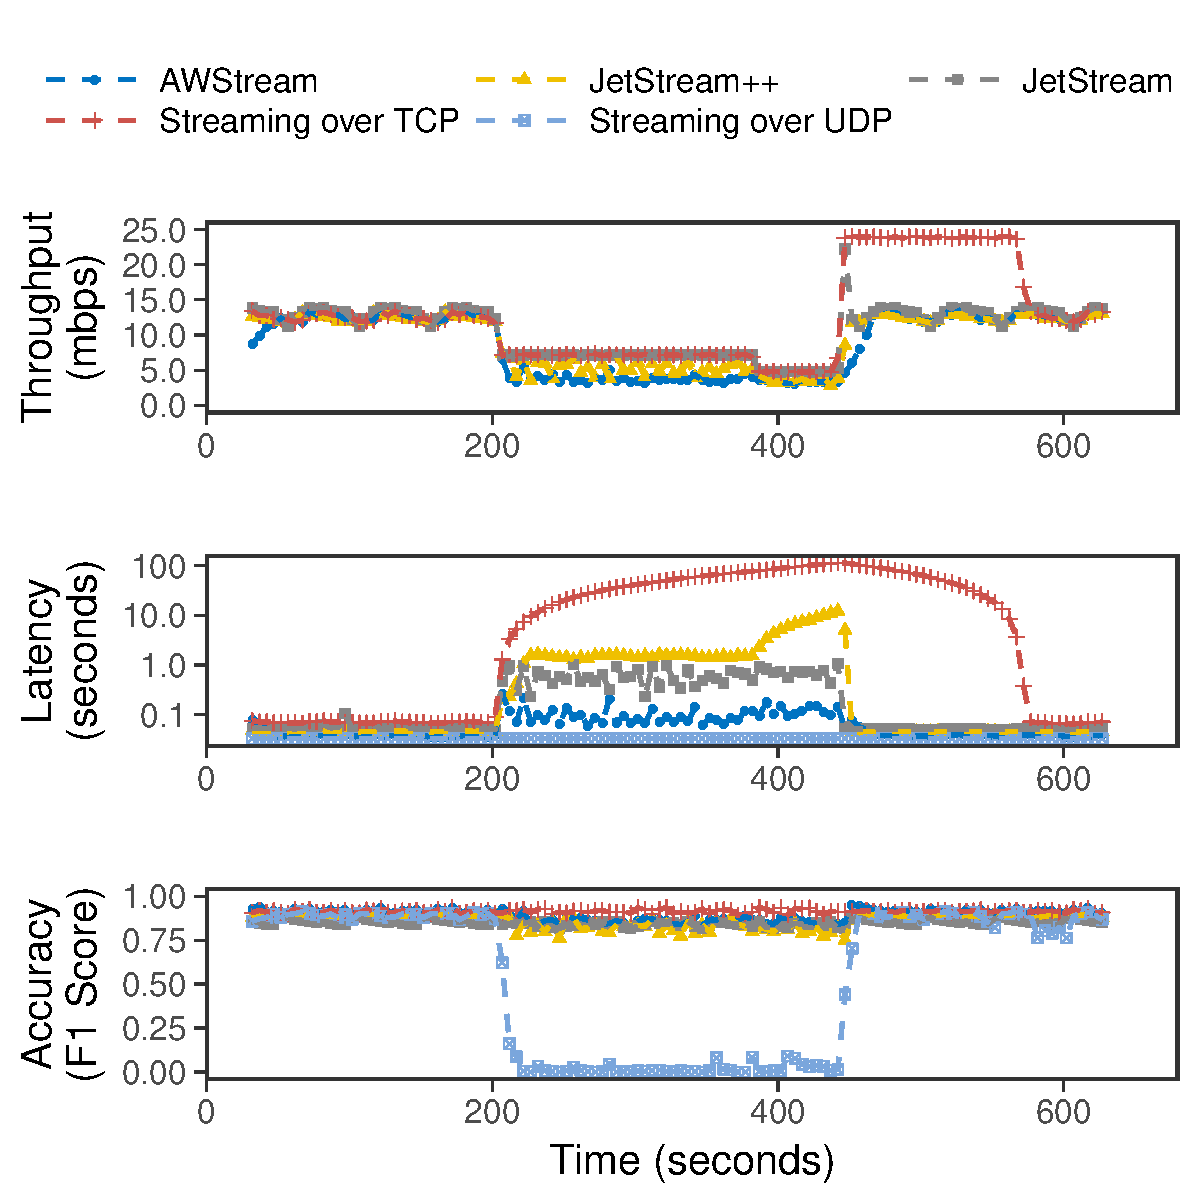
\includegraphics[width=\columnwidth]{figures/runtime_mot-timeseries.pdf}
    \caption{PD's runtime behavior with a time-series plot: throughput (top),
      showing the effect of bandwidth shaping; latency (middle) in log scale;
      and accuracy (bottom).}
    \label{fig:pd-runtime-timeseries}
  \end{subfigure}
  \vspace{1em}
  \\
  \begin{subfigure}[t]{\columnwidth}
    \centering
    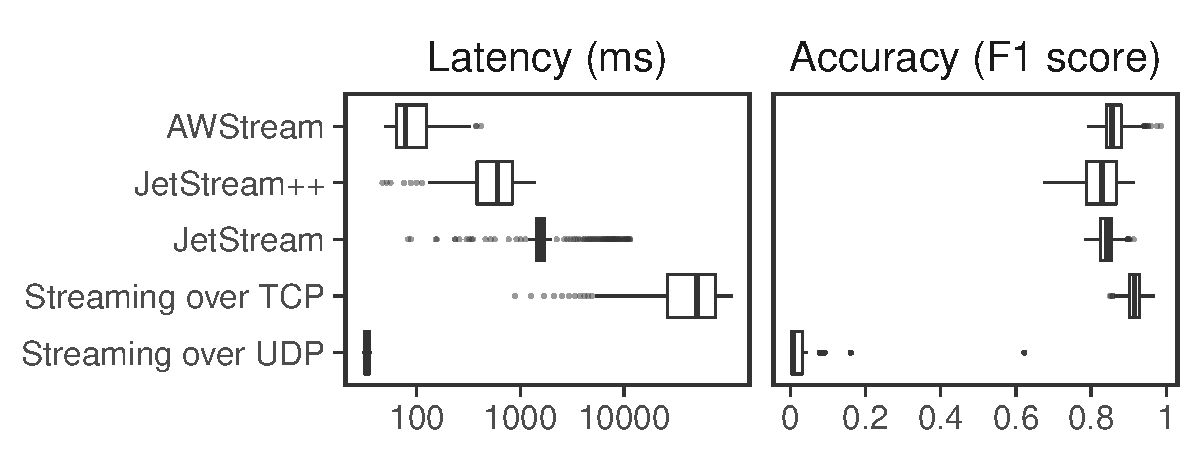
\includegraphics[width=\columnwidth]{figures/runtime_mot-boxplot.pdf}
    \caption{PD's performance summary of latency and accuracy during the traffic
      shaping (between t=200s and t=440s).}
    \label{fig:pd-runtime-boxplot}
  \end{subfigure}
  \caption{PD runtime evaluation.}
  \label{fig:pd-runtime}
  \vspace{-0.5em}
\end{figure}

\begin{figure}[t]
  \begin{subfigure}[t]{\columnwidth}
    \centering
    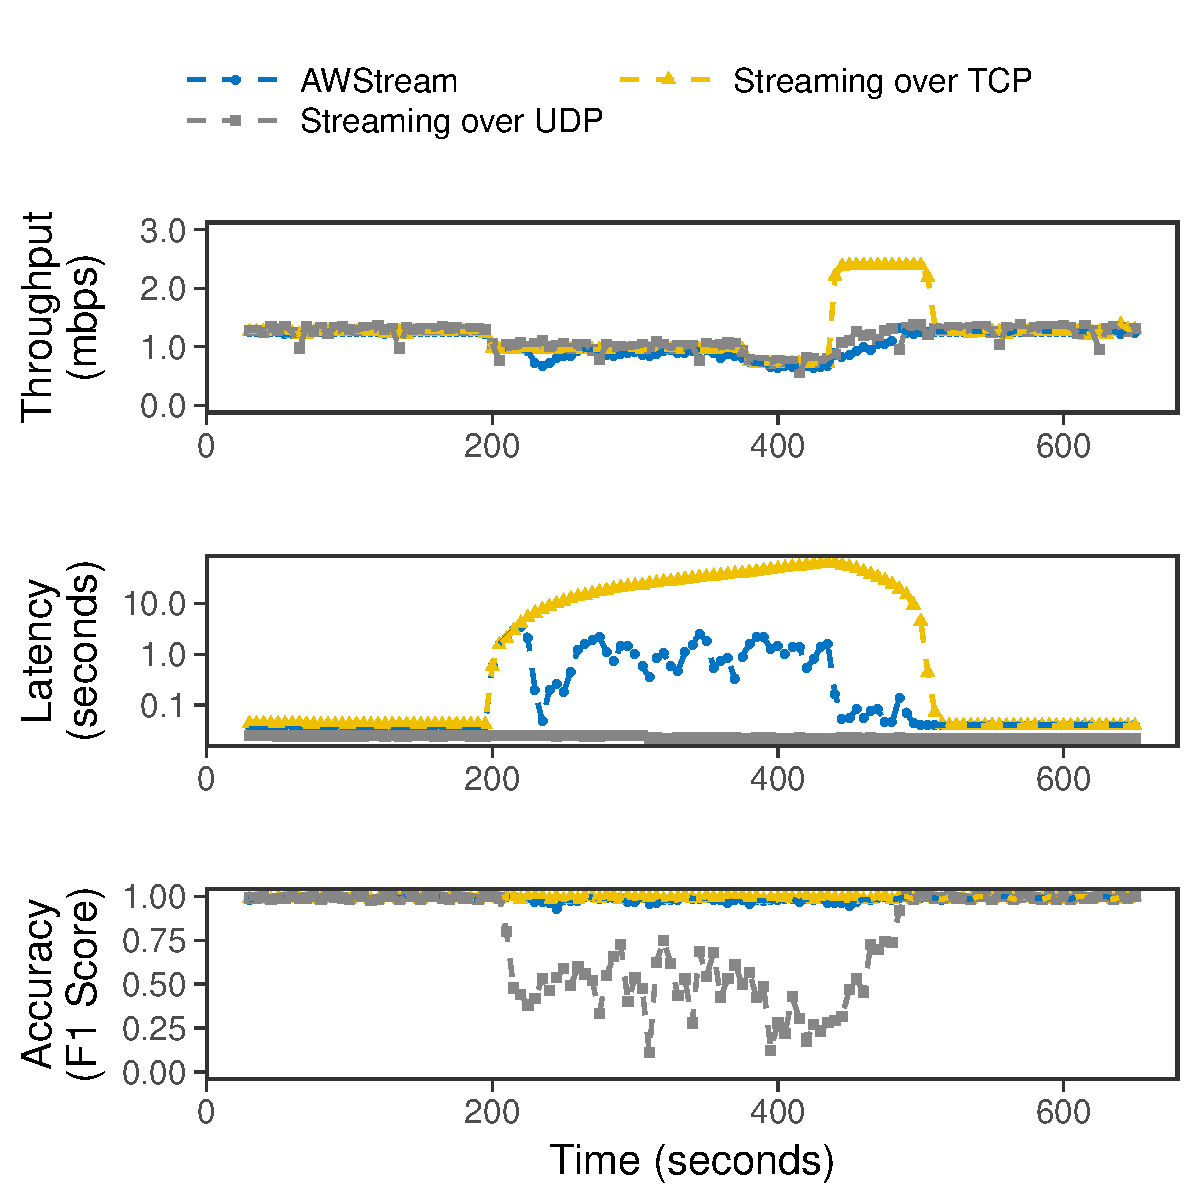
\includegraphics[width=\columnwidth]{figures/runtime_tk-timeseries.pdf}
    \caption{TK's runtime behavior with a time-series plot: throughput (top),
      showing the effect of bandwidth shaping; latency (middle) in log scale;
      and accuracy (bottom).}
    \label{fig:tk-runtime-timeseries}
  \end{subfigure}
  \vspace{1em}
  \\
  \begin{subfigure}[t]{\columnwidth}
    \centering
    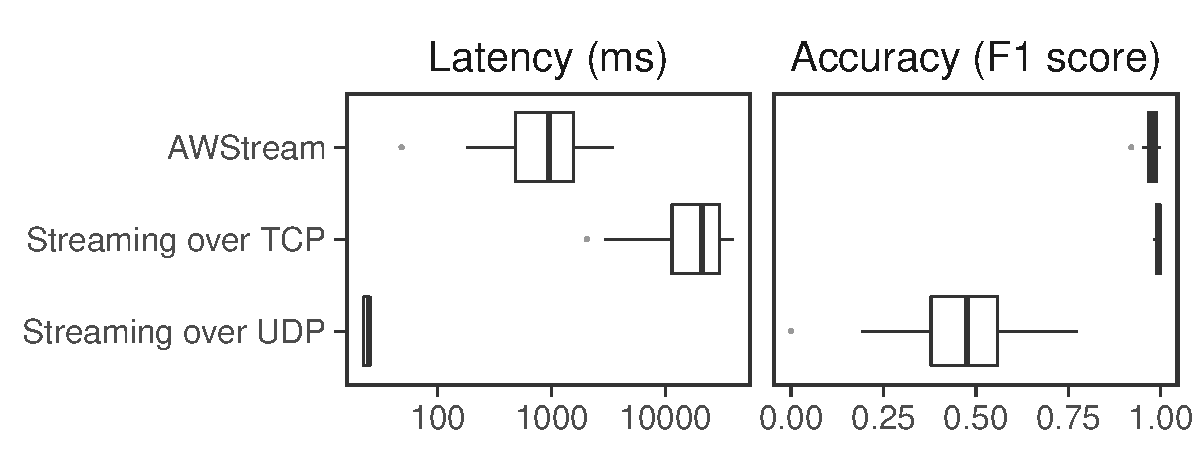
\includegraphics[width=\columnwidth]{figures/runtime_tk-boxplot.pdf}
    \caption{TK's performance summary of latency and accuracy during the traffic
      shaping (between t=200s and t=440s).}
    \label{fig:tk-runtime-boxplot}
  \end{subfigure}
  \caption{TK runtime evaluation.}
  \label{fig:tk-runtime}
  \vspace{-0.5em}
\end{figure}

\paraf{Pedestrian Detection.} The setup for PD is the same with AR: three Amazon
EC2 as clients and one as server. The maximal configuration $c_{\max}$ is
1920x1080 resolution, \(10~\text{FPS}\) and a quantization of 20; it consumes
about \SI{12}{Mbps}. For PD, \sysname{} learns that frame rate is less important
than resolution. It favors 10FPS with 1080p instead of 30FPS with 900p as in AR.

When running experiments, we use the same bandwidth shaping schedule as we used
for AR. Baselines are also the same: Streaming over TCP, streaming over UDP,
JetStream, JetStream++, and HLS.

\autoref{fig:pd-runtime} shows the runtime behavior in both time series
(throughout the experiment) and box plot (between t=200s and t=440s).  Most
observations we made in the main paper are the same here: $(i)$~Streaming with
TCP has the highest accuracy (median 92\%) at a cost of high
latency. $(ii)$~Streaming with UDP has the lowest bounded latency but the
accuracy is too low. $(iii)$~HLS incurs a latency of 2-3 seconds due to
chunking, buffering, and client fetching; its accuracy in PD is quite poor
because HLS reduces latency and encoding quality. $(iv)$~JetStream and
JetStream++ can balance latency and accuracy; but JetStream's manual policy is
unable to sustain \SI{5}{Mps} bandwidth, so its median latency is high
(\SI{1535}{\ms}); JetStream++'s latency is lower (\SI{598}{\ms}) than JetStream,
but its accuracy (82\%) suffers from policy oscillation. \sysname{} is able to
achieve the lowest latency (\SI{78}{ms}) with small accuracy drop (86\%, 6\%
drop in comparison to TCP). In comparison to the state-of-the-art system
JetStream, \sysname{} improves the latency by 20$\times$ (from \SI{1535}{ms} to
\SI{78}{ms}) and accuracy by 1\% (from 84\% to 85\%).

\para{Top-K.} For TK, our logs are split into four groups. We then use four
Amazon EC2 as clients and one as server. The maximal configuration $c_{\max}$ is
$N=9750$ for \texttt{head} and $T=0$ for \texttt{threshold}; it consumes about
\SI{1.2}{Mbps}. Because the overall bandwidth consumption is much smaller than
video analytics, we change the bandwidth parameter for runtime evaluation:
during t=200-380s, we limit the bandwidth to \SI{750}{Kbps}; during t=380-440s,
the bandwidth is \SI{500}{Kbps}; the background limit is \SI{2.5}{Mpbs}.

We've only compared \sysname{} with two baselines: streaming over TCP and
streaming over UDP. For TCP baseline, we use \sysname{} but disable the
adaptation. For UDP baseline, we implemented a simple application
protocol---packetization and a custom header---so that the receiver can still
aggregate data in the presence of UDP packet loss. While JetStream provides a
Top-K implementation, it is based on Three-Phase Uniform Threshold (TPUT) and
not suitable for low-latency Top-K monitoring. We quote from the original paper
of TPUT~\cite{cao2004efficient}, \textit{``in our target environments the query
  is asked hourly or daily. The intervals between the queries are typically long
  enough that the top-k objects have changed completely.''} In addition, we did
not implement our Top-K pipeline (\autoref{fig:topk}) with JetStream because
video analytical applications suffice the purpose of comparison.

\autoref{fig:tk-runtime} shows the evaluation results for the Top-K
application. Streaming over TCP has the highest accuracy (\textasciitilde
99.7\%) but the worst latency (up to 40 seconds). Streaming over UDP has the
lowest latency but its accuracy is the worst (\textasciitilde 52\%). \sysname{}
achieves low latency (\textasciitilde 1.1 second) and high accuracy
(\textasciitilde 98\%) simultaneously. Notice that because TK's source generates
data every second after the \texttt{Window} operation, one object in the queue
leads to one second latency. \sysname{} manages to avoid queues for most times.

\subsection{Performance with Various Network Delays}
\label{sec:various-rtt}

\sysname{} targets at wide area whose key characteristic is the large variation
in latency~\cite{li2010cloudcmp}. While we've conducted experiments using
real-world setup on Amazon EC2, the latency between EC2 sites is relatively low.
To evaluate how \sysname{} performs with increased network delays, we conducted
another experiment with one pair of client and server under different network
conditions. We use \texttt{netem} to add delays in addition to our bandwidth
shaping. The additional one-way delays ranges from 0 to \SI{250}{ms}, following
a normal distribution where the variation is 10\% of the added delay, e.g.
$250\pm 25\text{ms}$. We add delays in both direction, so the added RTT can be
as high as \SI{500}{ms}.

\begin{figure}
  \centering
  \includegraphics[width=.88\columnwidth]{figures/runtime_darknet-bench.pdf}
  \vspace{-0.5em}
  \caption{\sysname{} maintains low latency and high accuracy under different
    network delay conditions.}
  \label{fig:ar-rtt}
  \vspace{-0.5em}
\end{figure}

\autoref{fig:ar-rtt} shows the runtime behavior with various added network
delays. While the latency increases with the added delay, \sysname{} mostly
manages to achieve sub-second latency for all conditions. We see a higher
variation in latency and more outliers as network delay increases. This is
caused by a slow congestion detection when the RTT is high. In terms of
accuracy, because \sysname{} mostly stays in \texttt{Steady} state and accuracy
only depends on the level of degradation, \sysname{} achieves similar accuracy
for different network delays.

\subsection{Resource Allocation and Fairness}
\label{sec:multi-task-alloc}

\begin{figure}
  \centering
  \begin{subfigure}[t]{0.7\columnwidth}
    \centering
    
\includegraphics[width=\textwidth]{figures/multitask-legend.pdf}
  \end{subfigure}
  \\
  \vspace{0.4em}
  \begin{subfigure}[t]{0.45\columnwidth}
    \centering
    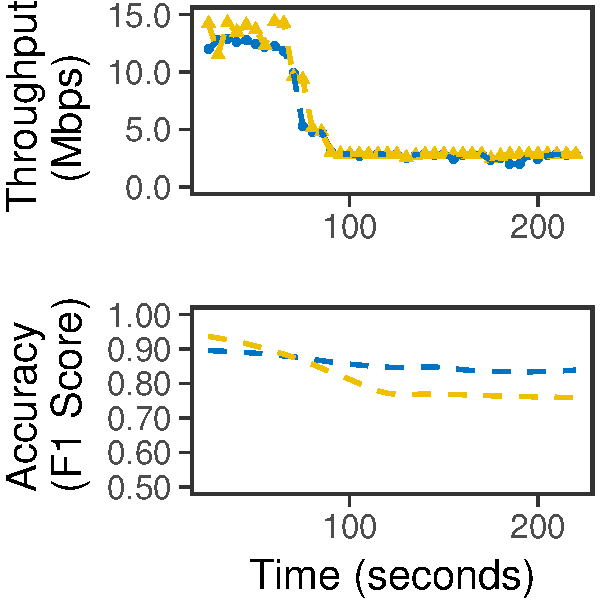
\includegraphics[width=\textwidth]{figures/multitask-left.pdf}
    \caption{Resource Fairness}
    \label{fig:eq-bw}
  \end{subfigure}
  \hfill
  \begin{subfigure}[t]{0.45\columnwidth}
    \centering
    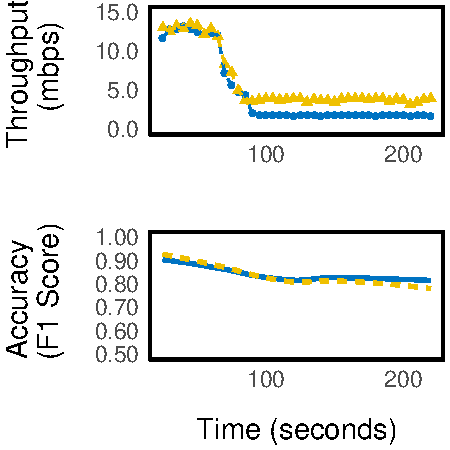
\includegraphics[width=\textwidth]{figures/multitask-right.pdf}
    \caption{Utility Fairness}
    \label{fig:eq-acc}
  \end{subfigure}
  \caption{\sysname{} supports a variety of resource allocation schemes:
    resource fairness (a) and utility fairness (b).}
  \label{fig:multitask}
  \vspace{-0.5em}
\end{figure}

We evaluate resource allocations with two applications. In this way, the result
also covers the case of a single application, and can generalize to more
applications.

We choose AR and PD as the example applications.  The clients and servers of
both applications are co-located so that they share the same bottleneck
link. The experiment starts with sufficient bandwidth. At t=60s, we start
traffic shaping to limit the total bandwidth to \SI{6}{Mbps}. When we allocate
resource equally between two applications (\autoref{fig:eq-bw}), each
application gets \SI{3}{Mbps}. Under this condition, PD runs with a higher
accuracy of 85\% while AR only achieves 77\%. In addition to resource fairness,
\sysname{} supports utility fairness: it chooses configurations that maximize
the minimal accuracy. In this experiment, PD receives \SI{2}{Mbps} and AR
receives \SI{4}{Mbps}; and both achieve 80\% accuracy (\autoref{fig:eq-acc}).

%%% Local Variables:
%%% mode: latex
%%% TeX-master: "../awstream"
%%% End:

%% LocalWords: TK PD runtime JetStream AR alloc YOLO dataset outliers
%% LocalWords: makespan subsec mins tcp boxplot geo HLS ffmpeg geforce
%% LocalWords: HLS PD's mis bw quantization RTSP RTP GPUs parallelization
%% LocalWords: eq netem resizes RTTs parallelize LFS UDP GTX analytics
%% LocalWords: FFmpeg GeForce HLS's JetStream's TK's
\section{Discussion and Future work}
\label{sec:discussion}

We have presented \sysname{}, a stream processing system achieving low latency
and high accuracy for the wide area. This section discusses limitations and
future work.

\para{Reducing developer effort.} While \sysname{} focuses on reducing developer
effort from tedious manual policy construction, there are still
application-specific aspects for developers: writing appropriate \maybe{} calls,
providing training data, and specifying the accuracy function. Because
\sysname{}'s API is extensible, we plan to build more libraries for common
degradation operators and accuracy functions, similar to machine learning
libraries.

\para{Fault-tolerance and failure recovery.} \sysname{} tolerates bandwidth
variation but not network partition or host failure. Although servers within
data centers can handle faults in existing systems, such as Spark
Streaming~\cite{zaharia2013discretized}, it is difficult to make edge clients
failure-oblivious.  We leave failure detection and recovery as a future work.

\para{Profile modeling.} \sysname{} currently does not model $B(c)$/$A(c)$. It
performs an exhaustive search when profiling. While parallelism and sampling
techniques can speed this up, \sysname{} can benefit further from statistical
techniques. Bayesian Optimization~\cite{snoek2012practical}, as demonstrated by
CherryPick~\cite{alipourfard2017cherrypick}, models black-box functions and
speeds up profiling by searching for near-optimal configurations. We plan to
explore this direction to improve our profiling.

% \para{Expressiveness}: Our \maybe{} APIs allow an easy integration with
% existing stream processing systems. While it follows the operator model,
% combined with other operators, this is expressive enough. We've presented
% three applications in this paper; and we are implement more application using
% this framework to understand the expressiveness better.

% \para{Context detection.} \sysname{} is currently limited to one profile: the
% offline profiling generates the default profile and the online profiling
% updates the single profile continuously.  Real-world applications may produce
% data with a multi-modal distribution, where the model changes upon context
% changes, such as indoor versus outdoor. Therefore, one possible optimization
% to \sysname{} is to allow multiple profiles for one application, detect
% context changes, and use the profile that best matches the current data
% distribution.  Switching contexts could reduce, or even eliminate, the
% overhead of online profiling.

\para{Predicting bandwidth changes.} Our runtime currently does not predict
future bandwidth. While reacting to bandwidth changes is enough to achieve
sub-second latency, if \sysname{} can accurately predict future bandwidth, we
expect further improvements such as no latency spikes or a simplified runtime
design. Techniques such as model predictive control (MPC) have improved QoE in
video streaming with throughput prediction~\cite{yin2015control}; we plan to
investigate using MPC in \sysname{} as a future work.

%%% Local Variables:
%%% mode: latex
%%% TeX-master: "../awstream"
%%% End:

\section{Related Work}
\label{sec:related-work}

\paraf{JetStream.} JetStream is the first to use degradation to reduce latency
for wide-area streaming analytics. Compared to JetStream, \sysname{} makes five
major contributions: $(1)$~a novel API design to specify degradation in a simple
and composable way; $(2)$~automatic offline profiling to search for
Pareto-optimal configurations; $(3)$~online profiling to address model drift;
$(4)$~an improved runtime system achieving sub-second latency (comparison in
\autoref{sec:runtime-adaptation}); $(5)$~support for different resource
allocation policies for multiple applications.

\para{Stream Processing Systems.} Early streaming
databases~\cite{abadi2005design, chandrasekaran2003telegraphcq} have explored
the use of dataflow models with specialized operators for stream
processing. Recent research projects and open-source
systems~\cite{akidau2013millwheel, toshniwal2014storm, sanjeev2015twitter,
  zaharia2013discretized, carbone2015apache} primarily focus on fault-tolerance
in the context of a single cluster. When facing back pressure,
Storm~\cite{toshniwal2014storm}, Spark Streaming~\cite{zaharia2013discretized}
and Heron~\cite{sanjeev2015twitter} throttle data ingestion; Apache
Flink~\cite{carbone2015apache} uses edge-by-edge back-pressure techniques
similar to TCP flow control; Faucet~\cite{lattuada2016faucet} leaves the flow
control logic up to developers.  While our work has a large debt to prior
streaming work, \sysname{} targets at the wide area and explicitly explores the
trade-off between data fidelity and freshness.

\cameraready{\para{Approximate Analytics.} The idea of degrading computation
  fidelity for responsiveness is also explored elsewhere, such as SQL
  queries~\cite{agarwal2013blinkdb, ananthanarayanan2014grass}, real-time
  processing~\cite{farrell2016meantime}, and video processing within large
  clusters~\cite{zhang2017live}. They employ techniques such programming
  language support~\cite{sampson2011enerj},
  sampling~\cite{garofalakis2001approximate}, sketches~\cite{cormode2011sketch},
  and online aggregation~\cite{hellerstein1997online}.}  The trade-off between
available resource and application accuracy is a common theme among all these
systems. \sysname{} targets at wide-area streaming analytics, an emerging
application domain especially with the advent of IoT\@.

\para{WAN-Aware Systems.} Geo-distributed systems need to cope with high latency
and limited bandwidth. While some systems assume the network can prioritize a
small amount of critical data under congestion~\cite{cho2012surviving}, most
systems reduce data sizes in the first place to avoid congestion
(e.g.,~LBFS~\cite{muthitacharoen2001low}). Over the past two years, we have seen
a plethora of geo-distributed analytical
frameworks~\cite{vulimiri2015wananlytics, vulimiri2015global, pu2015low,
  kloudas2015pixida, viswanathan2016clarinet} that incorporate heterogeneous
wide-area bandwidth into query optimization to minimize data movement. While
effective in speeding up analytics, these systems focus on batch tasks such as
MapReduce jobs or SQL queries. Such tasks are often executed infrequently and
without real time constrain. In contrast, \sysname{} processes streams
continuously in real time.

%% - Pixida~\cite{kloudas2015pixida} minimizes data movement across inter-DC
%% links by solving a traffic minimization problem in data analytics.

%% - Iridium~\cite{pu2015low} optimizes data and task placement jointly to
%% achieve an overall low latency goal.

%% - Clarinet~\cite{viswanathan2016clarinet} incorporate bandwidth information
%% into query optimizer to reduce data transfer.

%% WheelFS~\cite{stribling2009flexible}

%% Geode~\cite{vulimiri2015global} develops input data movement and join
%% algorithm selection strategies to minimize WAN bandwidth usage.

%% WANalytics~\cite{vulimiri2015wananlytics} focuses on batch analytics.

%% SWAG~\cite{hung2015scheduling} coordinates compute task scheduling across
%% DCs.

%% \cite{heintz2015towards} discusses the complex trade-offs involved in
%% wide-area analytics.

\para{(Adaptive) Video Streaming.} Multimedia streaming protocols
(e.g.,~RTP~\cite{schulzrinne2006rtp}) aim to be fast instead of reliable. While
they can achieve low latency, their accuracy can be poor under congestion.
Recent work has moved towards HTTP-based protocols and focused on designing
adaptation strategy to improve QoE, as in research~\cite{mao2017neural,
  sun2016cs2p, yin2015control} and industry (HLS~\cite{pantos2016http},
DASH~\cite{michalos2012dynamic, sodagar2011mpeg}). These adaptation strategies
are often pull-based: client keeps checking the index file for changes. And
clients have to wait for the next chunk (typically 2-10 seconds). In addition,
as we have shown in \autoref{sec:runtime-adaptation}, their adaptation is a poor
match for analytics that rely on image details (e.g.,~6\% accuracy for PD). In
contrast, \sysname{} learns an adaptation strategy for each application (also
not limited to video analytics); and the runtime is optimized for low latency.

\para{QoS.} Most QoS work~\cite{ferrari1990scheme, shenker1994integrated,
  shenker1995fundamental} in the 1990s focuses on network-layer solutions that
are not widely deployable. \sysname{} adopts an end-host application-layer
approach ready today for WAN. For other application-layer
approaches~\cite{vandalore2001survey}, \sysname{}'s API can incorporate their
techniques, such as encoding the number of layers as a knob to realize the
layered approach in Rejaie et al~\cite{rejaie2000layered}. Fundamentally,
\sysname{} does not provide hard QoS guarantees; instead \sysname{} maximizes
achievable accuracy (application performance) and minimizes latency (system
performance) with respect to bandwidth constraints: a multidimensional
optimization.

%% TCP, for example, adapts to available bandwidth by controlling the congestion
%% window with AIMD~\cite{jacobson1988congestion}.  Previous work has proposed
%% modifications to TCP for specific contexts. For streaming over TCP, Goel et
%% al.~\cite{goel2008low} proposes adaptive buffer-size tuning. For the cloud,
%% Adaptive TCP~\cite{wu2013adaptive} proposes to modify the congestion control
%% behavior based on flow size for the cloud.

% \para{Scheduling and allocation:} Resource allocations in the cloud is how to
% efficiently allocate tasks.  In the wide area, we face fundamental limit that
% therefore degradation is more effective. For multiple tasks, Existing
% allocations are for resources without considering application trade-offs.
% MediaNet~\cite{hicks2003user} uses both local and online global resource
% scheduling to improve user performance and network utilization, and adapts
% without requiring underlying support for resource
% reservations. VideoStorm~\cite{zhang2017live} primarily focuses on cluster
% resource allocation among video queries. For wide-area, the resource
% allocation is limited. We do not control the capacity; but still we can
% allocate the available bandwidth.

% Performance modeling: CherryPick~\cite{alipourfard2017cherrypick},
% Ernest~\cite{venkataraman2016ernest}.
%% Dolly~\cite{ananthanarayanan2013effective}.
%% \para{Program Synthesis:}

%%% Local Variables:
%%% mode: latex
%%% TeX-master: "../awstream"
%%% End:

%% LocalWords: JetStream analytics composable runtime Borealis TelegraphCQ
%% LocalWords: dataflow MillWheel Flink TCP BlinkDB VideoStorm IoT geo LBFS
%% LocalWords: WANalytics Pixida MapReduce RTP HLS QoE VoD QoS deployable Rejaie
%% LocalWords: et al

\section{Conclusion}
\label{sec:conclusion}

The emerging class of wide-area streaming analytics faces the challenge of
scarce and variable bandwidth. Developers need to make a tradeoff between data
freshness and fidelity. While it is easy to build applications for either high
accuracy or low latency, achieving both simultaneously is challenging. Previous
approaches using manual policies end up with sub-optimal
performance. Application-specific optimizations do not generalize to cover the
variety and scales of potential applications.

In this paper, we present \sysname{}, a stream processing system for a wide
variety of applications by enabling developers to customize degradation
operations with \maybe{} API. Our automatic profiling tool generates an accurate
profile that characterizes the tradeoff between bandwidth consumption and
application accuracy. The profile allows the runtime to react with
precision. Evaluations with three applications show that \sysname{} achieves
sub-second latency with nominal accuracy drop. \sysname{} enables resilient
execution of wide-area streaming analytics with minimal developer effort.

%%% Local Variables:
%%% mode: latex
%%% TeX-master: "../awstream"
%%% End:


% \appendix

% \section{WAN Bandwidth Characteristics}

% \autoref{fig:aws-bandwidth} shows the available bandwidth between Amazon EC2
% servers (Tokyo, Ireland, N. Virginia, N. California) in our day-long
% measurements. Most inter-continental links (between Ireland and all others,
% between Tokyo and N. Virginia) have limited bandwidth (\textasciitilde
% \SI{50}{Mbps}). Other pairs exhibit large variations from \SI{10}{Mbps} up to
% \SI{150}{Mbps}.

% \begin{figure}
%   \centering
%   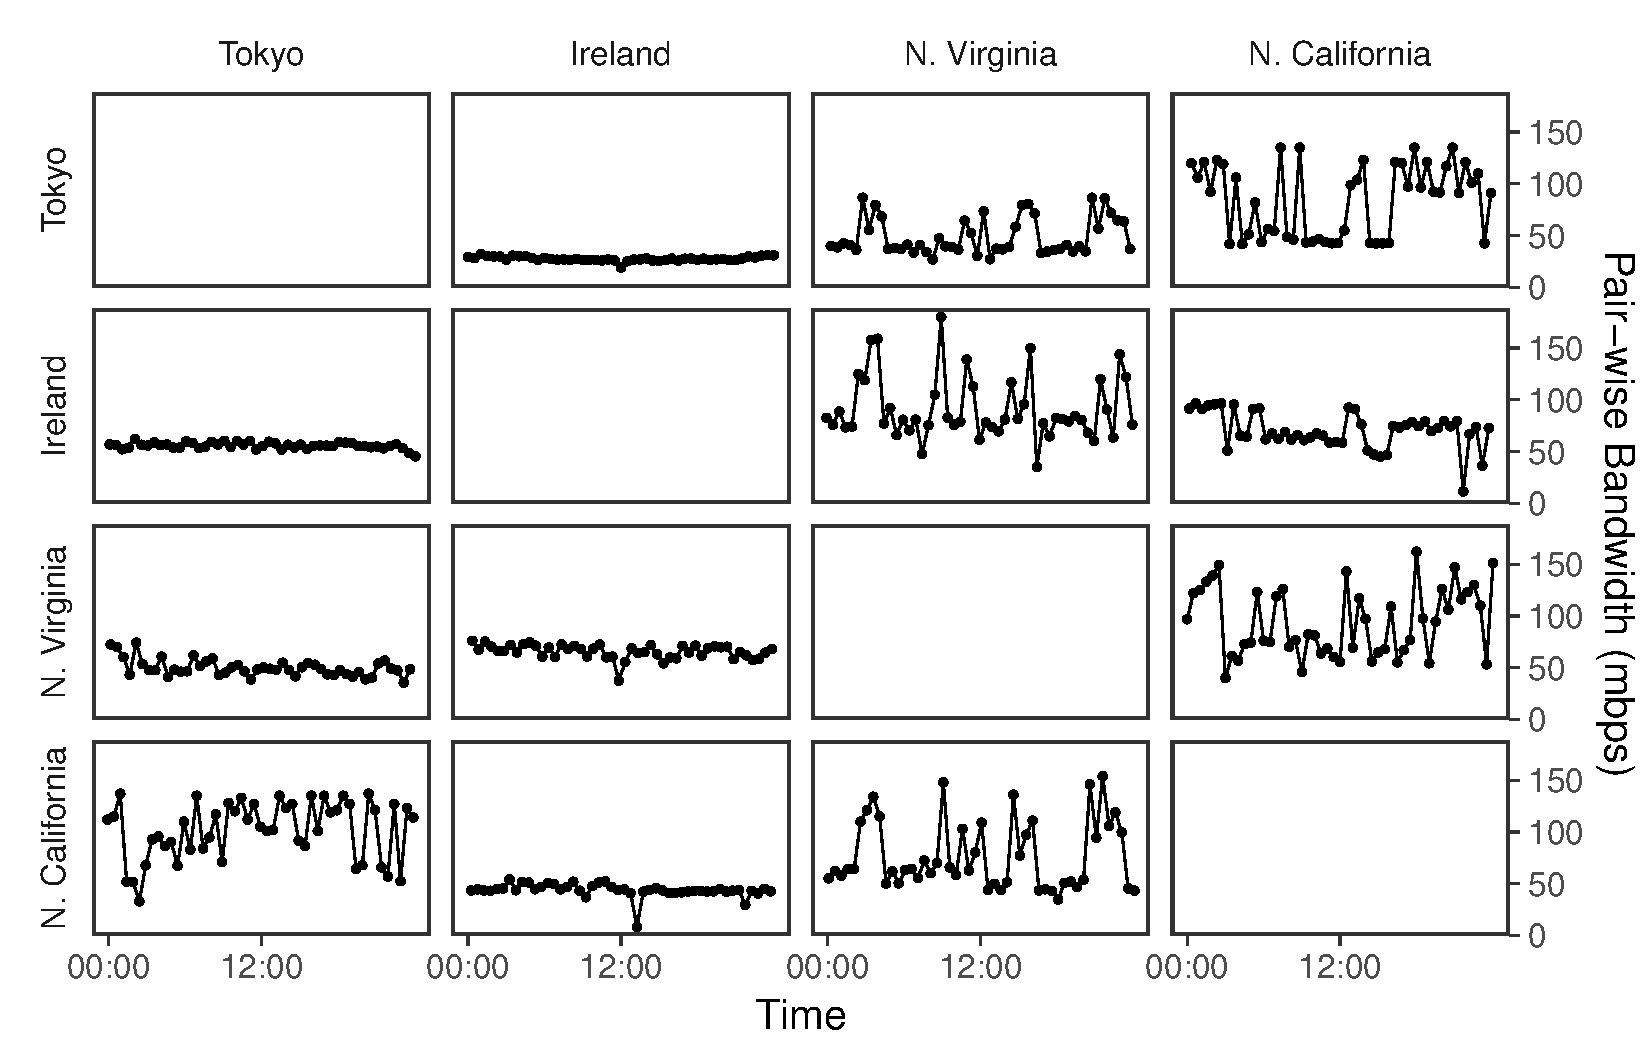
\includegraphics[width=\columnwidth]{figures/aws-bandwidth.pdf}
%   \caption{Pair-wise bandwidth in time series from our day-long measurements.}
%   \label{fig:aws-bandwidth}
% \end{figure}

\section{HLS Setup}
\label{appendix:hls-setup}

HTTP Live Streaming (HLS)~\cite{pantos2016http} represents a class of HTTP-based
media streaming protocols. Other protocols include Adobe HTTP Dynamic
Streaming~\cite{adobestreaming}, Microsoft Smooth
Streaming~\cite{zambelli2009iis}, and a newer vendor-independent standard
DASH~\cite{michalos2012dynamic, sodagar2011mpeg}. These adaptive streaming
protocols are widely adopted for both video-on-demand (VoD) and live streaming
(such as Periscope).

Our setup (\autoref{fig:hls}) resembles the setup of popular live streaming
services~\cite{wang2016anatomy}. Typical streaming servers set each chunk to be
2-10 seconds~\cite{mao2017neural, sun2016cs2p, wang2016anatomy}. For our low
latency streaming, we configured the chunk segment to be 1 second.

\para{Why HLS/DASH is a poor match for video analytics?} It's hard to achieve
ultra low latency using HLS/DASH: (1) HLS/DASH is pull-based: the client keeps
requesting for new chunks; (2) HLS/DASH uses chunking: shorter chunks enable a
lower latency, but induce a larger number of requests, and the chunk has to be
made ready before the client can start fetching. There are proposals to reduce
the latency, such as server push~\cite{wei2014low}, but they are still work in
progress. For some applications, the accuracy can also be poor if these videos
are limited to tuning resolution and encoding quality only, as demonstrated by
in our PD evaluation.

\begin{figure}[t]
  \centering
  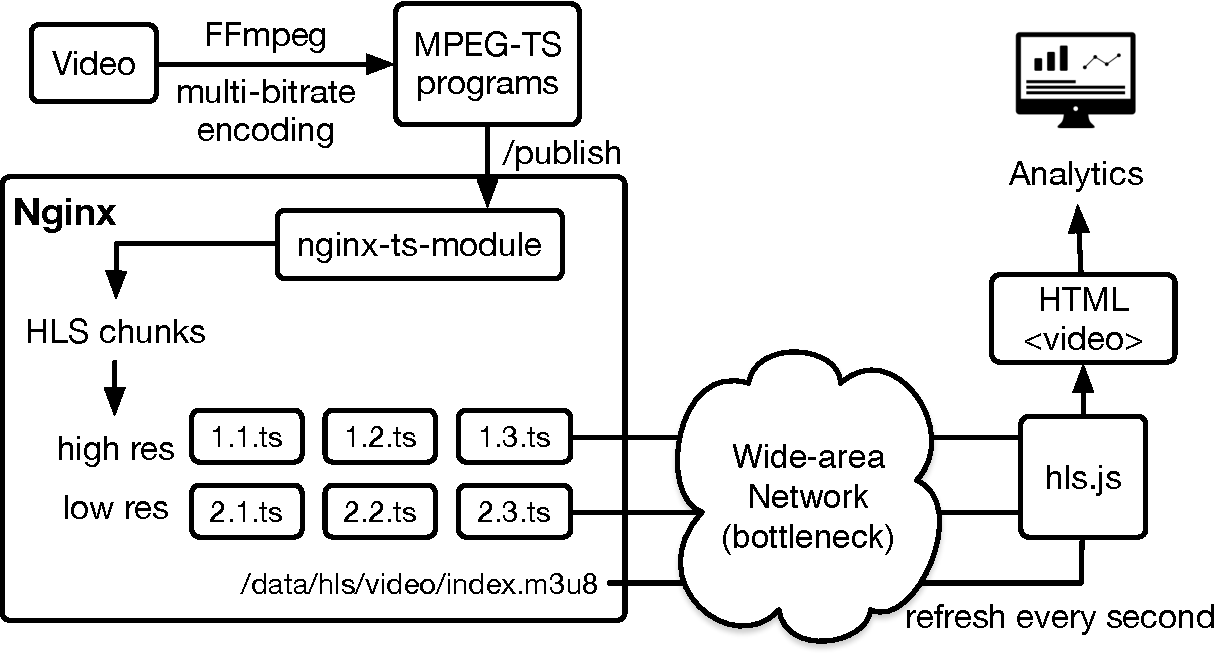
\includegraphics[width=\columnwidth]{figures/hls.pdf}
  \caption{HLS setup: (1)~FFmpeg encodes video with multiple bitrates and groups
    them into MPEG-TS programs;
    (2)~\texttt{nginx-ts-module}~\cite{nginx-ts-module} generates HLS chunks on
    the fly and stores them for nginx serving; (3)~the client (using
    \texttt{hls.js}~\cite{hls.js}) periodically fetches the latest index file
    (\texttt{index.m3u8}) and then downloads the right chunk according to
    network conditions.}
  \label{fig:hls}
\end{figure}

\section{JetStream++}
\label{appendix:jetstream++}

We modified the open source version of
JetStream\footnote{\url{https://github.com/princeton-sns/jetstream/}, commit
  bf0931b2d74d20fdf891669188feb84c96AF84.} in order to use our profile as its
manual policy. Because JetStream doesn't support simultaneous degradation across
multiple operators, we implemented a simple \texttt{VideoSource} operator that
understands how to change image resolutions, frame rate, and video encoding
quantization. At runtime, \texttt{VideoSource} queries congestion policy manager
and adjusts three dimensions simultaneously. This operator is then exposed to
the Python-implemented control plane. We call this modified version
JetStream++.\footnote{URL to our patch is elided for anonymity.}

%% https://github.com/nebgnahz/jetstream-clone/pull/2/files}

JetStream's code base is modular and extensible: the modifications include 53
lines for the header file, 171 lines for implementation, 75 lines for unit test,
and 49 lines of python as the application. While extending JetStream with our
profile is not challenging, JetStream++ performs degradation in a single
operator and loses the composability. We could modify JetStream to support
degradation across multiple operators, but that would require substantial
changes to JetStream. Using JetStream++ with our profile, the comparison is
enough to illustrate the difference between \sysname{}'s and JetStream's
runtime.

 % > summary(latency)
 %      Time        JetStream++        JetStream            HLS
 % Min.   :206.0   Min.   :  46.68   Min.   :   82.4   Min.   :1887
 % 1st Qu.:264.2   1st Qu.: 380.70   1st Qu.: 1435.7   1st Qu.:2320
 % Median :322.5   Median : 597.67   Median : 1534.9   Median :2623
 % Mean   :322.5   Mean   : 624.21   Mean   : 2629.2   Mean   :2610
 % 3rd Qu.:380.8   3rd Qu.: 831.75   3rd Qu.: 1688.1   3rd Qu.:2863
 % Max.   :439.0   Max.   :1388.79   Max.   :11489.3   Max.   :4227
 % NA's   :1       NA's   :1         NA's   :1         NA's   :1
 %
 % Streaming over TCP Streaming over UDP    AWStream
 % Min.   :   878.8   Min.   :29.70      Min.   : 48.35
 % 1st Qu.: 26176.3   1st Qu.:31.18      1st Qu.: 63.58
 % Median : 50679.0   Median :32.68      Median : 77.98
 % Mean   : 52130.4   Mean   :32.89      Mean   :105.56
 % 3rd Qu.: 76010.8   3rd Qu.:34.60      3rd Qu.:124.71
 % Max.   :111455.7   Max.   :36.30      Max.   :417.79
 % NA's   :1          NA's   :1          NA's   :1
 %%
 %% 20x over JetStream, 7.7x over JetStream++

 % > summary(accuracy)
 %      Time        JetStream++       JetStream           HLS
 % Min.   :206.0   Min.   :0.6735   Min.   :0.7822   Min.   :0.00000
 % 1st Qu.:264.2   1st Qu.:0.7871   1st Qu.:0.8247   1st Qu.:0.04077
 % Median :322.5   Median :0.8285   Median :0.8420   Median :0.06372
 % Mean   :322.5   Mean   :0.8232   Mean   :0.8395   Mean   :0.09429
 % 3rd Qu.:380.8   3rd Qu.:0.8667   3rd Qu.:0.8531   3rd Qu.:0.09346
 % Max.   :439.0   Max.   :0.9148   Max.   :0.9130   Max.   :0.69602
 % NA's   :1       NA's   :1        NA's   :1        NA's   :1
 % Streaming over TCP Streaming over UDP      AWStream
 % Min.   :0.8502     Min.   :-0.0000985   Min.   :0.7899
 % 1st Qu.:0.9012     1st Qu.: 0.0021567   1st Qu.:0.8405
 % Median :0.9150     Median : 0.0068409   Median :0.8552
 % Mean   :0.9150     Mean   : 0.0314461   Mean   :0.8622
 % 3rd Qu.:0.9295     3rd Qu.: 0.0312727   3rd Qu.:0.8805
 % Max.   :0.9697     Max.   : 0.6220806   Max.   :0.9853
 % NA's   :1          NA's   :1            NA's   :1
 %%
 %% 6% drop, 1% increase over JetStream

% > summary(latency)
%       Time       Streaming over TCP Streaming over UDP    AWStream
%  Min.   :210.0   Min.   : 2036      Min.   :22.29      Min.   :  48.03
%  1st Qu.:251.2   1st Qu.:11438      1st Qu.:22.42      1st Qu.: 485.08
%  Median :292.5   Median :21014      Median :24.78      Median : 946.45
%  Mean   :292.5   Mean   :20590      Mean   :23.85      Mean   :1145.05
%  3rd Qu.:333.8   3rd Qu.:29662      3rd Qu.:24.87      3rd Qu.:1557.20
%  Max.   :375.0   Max.   :39434      Max.   :24.98      Max.   :3509.99
% > summary(accuracy)
%       Time       Streaming over TCP Streaming over UDP    AWStream
%  Min.   :210.0   Min.   :0.9808     Min.   :0.1097     Min.   :0.9284
%  1st Qu.:251.2   1st Qu.:0.9892     1st Qu.:0.4467     1st Qu.:0.9694
%  Median :292.5   Median :0.9967     Median :0.5329     Median :0.9800
%  Mean   :292.5   Mean   :0.9928     Mean   :0.5236     Mean   :0.9786
%  3rd Qu.:333.8   3rd Qu.:0.9977     3rd Qu.:0.6063     3rd Qu.:0.9883
%  Max.   :375.0   Max.   :0.9991     Max.   :0.7981     Max.   :0.9991
%
% subsecond latency, 2% drop

% \section{HTTP Live Streaming}
\label{appendix:hls}

\begin{figure*}[t]
  \centering
  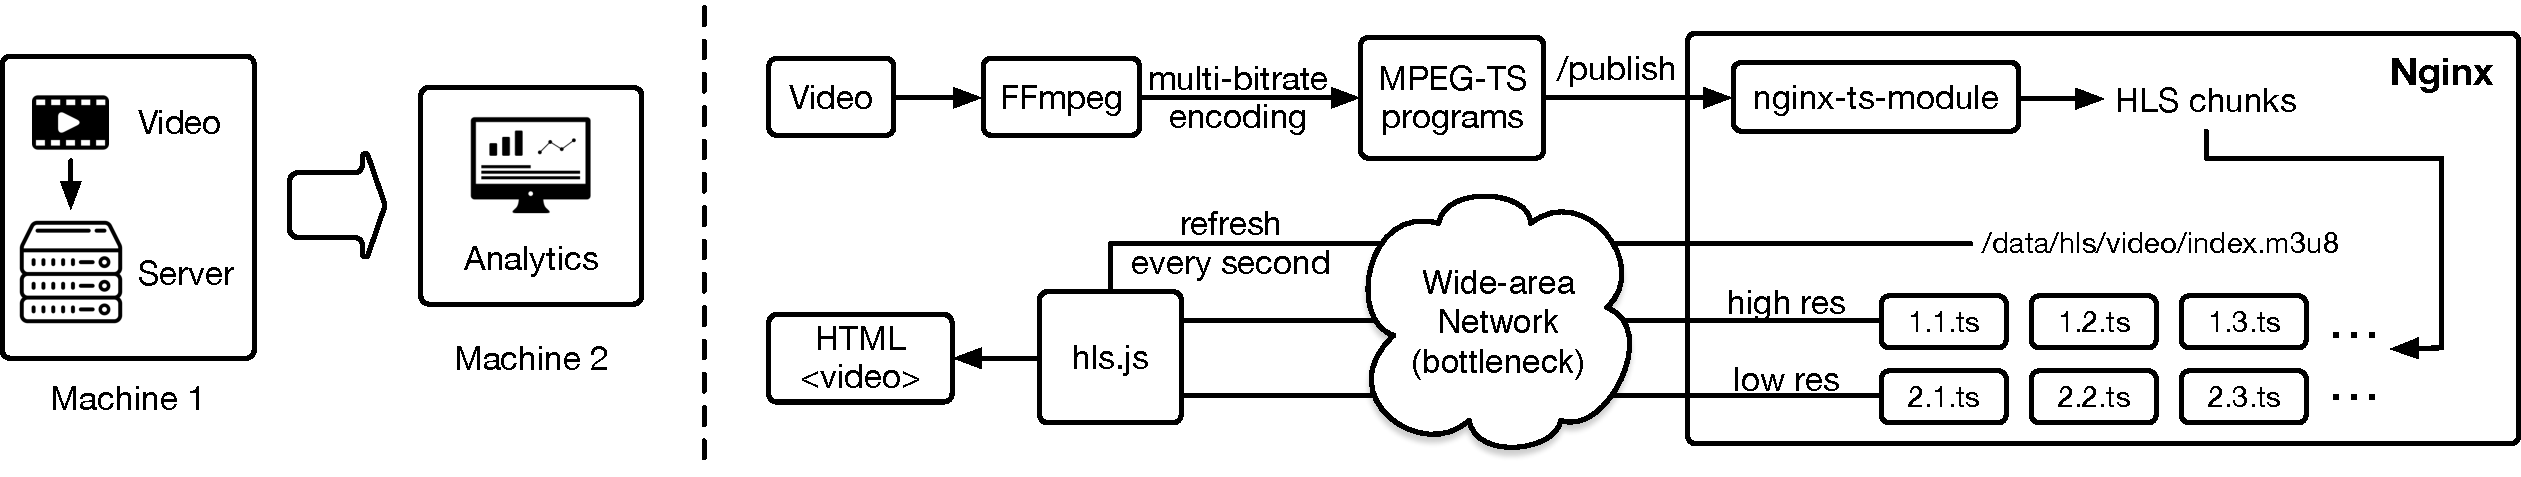
\includegraphics[width=\textwidth]{figures/hls-arch.pdf}
  \caption{HLS setup. (Left) High-level overview: machine 1 generates a video
    and stores it in the server; machine 2 fetches the data and performs
    analytics. (Right) Detailed view: (1)~FFmpeg encodes video with multiple
    bitrates and groups them into MPEG-TS programs; (2)~\texttt{nginx-ts-module}
    then generates HLS chunks on the fly and stores them for nginx serving;
    (3)~the client (using \texttt{hls.js}) periodically fetches the latest index
    file (\texttt{index.m3u8}) and then downloads the right chunk according to
    network conditions.}
  \label{fig:hls-arch}
\end{figure*}

HTTP Live Streaming (HLS)~\cite{pantos2016http} represents a class of HTTP-based
media streaming protocols. Other protocols include Adobe HTTP Dynamic
Streaming~\cite{adobestreaming}, Microsoft Smooth
Streaming~\cite{zambelli2009iis}, and a newer vendor-independent standard
DASH~\cite{michalos2012dynamic, sodagar2011mpeg}. These adaptive streaming
protocols are widely adopted for both video-on-demand (VoD) and live streaming
(such as Periscope).

Our setup (\autoref{fig:hls-arch}) resembles the setup of popular live streaming
services~\cite{wang2016anatomy}. We first describe each component of our
setup. We then discuss why these protocols are a poor match for wide-area
streaming analytics, despite their adaptation capability.

\para{Video.} We use \texttt{FFmpeg} to encode the video with multiple bitrates:
all levels use 30FPS, but different resolutions and H.264 encoding quality. Our
experiment uses six different bitrates---900p, 720p, 540p, 360p, all with normal
encoding quality; and 720p, 540p, with low encoding quality. To simulate live
video streaming, we then use \texttt{FFmpeg} to re-publish the stream to an
Nginx web server that accepts MPEG-TS (MPEG transport stream).

\para{Server.} Our web server is a nginx server compiled with plugin
\texttt{nginx-ts-module}~\cite{nginx-ts-module} that receives MPEG-TS over HTTP,
produces live HLS and DASH chunks. It creates an index file \texttt{index.m3u8}
that describes the media stream. During live streaming, the file is updated
whenever new chunks arrive. And the client needs to fetch the newest version of
\texttt{index.m3u8} to find out about new chunks. Typical streaming servers set
each chunk to be 2-10 seconds~\cite{mao2017neural, sun2016cs2p,
  wang2016anatomy}. For our low latency streaming, we configured the chunk
segment to be 1 second.

\para{Analytics.} The HTTP client reads the index file and then fetches each
chunk based on available bandwidth. Our client uses \texttt{hls.js}
\cite{hls.js}, a JavaScript library that implements an HLS client. It directly
plays the video inside an HTML5 video element. To avoid invoking the graphical
front-end of a browser, we use Puppeteer~\cite{puppeteer}, a NodeJS library that
provides a high-level API to control headless Chrome. During the runtime
experiment, instead of playing the video, we record the metadata with each
received chunk: its size, timestamp, and the quality level. We perform an
offline analysis of the log files to calculate the throughput, latency, and
accuracy.

Notice that the client-server relationship is reversed in HLS and \sysname{}. In
HLS, the server hosts video source files; the client fetches videos and
plays/computes. In \sysname{}, the client generates videos and pushes frames to
the server; the server performs video analytics.

\vspace{0.5em}
\para{Why HLS/DASH is a poor match for video analytics?} It's hard to achieve
ultra low latency using HLS/DASH: (1) HLS/DASH is pull-based: the client keeps
requesting for new chunks; (2) HLS/DASH uses chunking: shorter chunks enable a
lower latency, but induce a larger number of requests, and the chunk has to be
made ready before the client can start fetching. There are proposals to reduce
the latency, such as server push~\cite{wei2014low}, but they are still work in
progress. For some applications, the accuracy can also be poor if these videos
are limited to tuning resolution and encoding quality only, as demonstrated by
in our PD evaluation.

%%% Local Variables:
%%% mode: latex
%%% TeX-master: "../awstream"
%%% End:


%%% Local Variables:
%%% mode: latex
%%% TeX-master: "../awstream"
%%% End:

%% LocalWords: Mbps analytics runtime JetStream OpenCV YOLO pre GStreamer appsrc
%% LocalWords: appsink zerolatency quantization dataset SVM geo topk VideoSource
%% LocalWords: JetStream's composability TK TCP UDP HLS FFmpeg bitrates nginx
%% LocalWords: packetization TPUT topk NodeJS metadata timestamp Mbps Kbps
%% LocalWords: aws PD's TK's hls js VoD awstream tk fdf feb
% \begin{acks}
  This work was supported in part by the TerraSwarm Research Center, one of six
  centers supported by the STARnet phase of the Focus Center Research Program
  (FCRP) a Semiconductor Research Corporation program sponsored by MARCO and
  DARPA.

  The authors would like to thank Kaifei Chen and Pan Hu for providing feedback
  to an early version of this manuscript.
\end{acks}

%%% Local Variables:
%%% mode: latex
%%% TeX-master: "awstream"
%%% End:


\bibliographystyle{ACM-Reference-Format}
% \def \bibfont {\normalsize}
\bibliography{awstream}

\balance

\end{document}

%%% Local Variables:
%%% mode: latex
%%% TeX-master: t
%%% End: